\section{Performance}
\label{sec:Performance}

  A high statistics Monte Carlo simulation was used in order to measure the reconstruction efficiency and resolution of the implemented track-finding and track-fitting algorithms. It was necessarily Monte Carlo based in order to compare the reconstructed events to the simulated truth, thereby highlighting any inefficiencies and inaccuracies within the algorithms, without any additional noise or biases.

  The fitted transverse positions, $(x,y)$, and momenta, $(p_x, p_y, p_z)$, were compared to the Monte Carlo truth on an event-by-event basis. The reconstruction of the Monte Carlo data followed the same requirements that are used for the real data reconstruction. The Monte Carlo truth data was stored at every tracker plane to permit a direct comparison with the reconstructed data. All comparisons were made at the tracker reference surface. %the designated measurement location with the MICE cooling channel.

  An artificial beam was generated with uniform distributions for both the longitudinal and transverse momenta. This ensured that the results were not biased by the incoming beam distribution and that the full reconstructible phase space was probed with equal statistics. In order to remove unwanted non-physical particles, a cut was placed on the Monte Carlo truth data during the analysis phase to eliminate tracks with a high incoming angle. Tracks with a gradient ($p_t/p_z$) greater than $0.5$ were rejected from the analysis.

  \subsection{Track Finding Efficiency}
  \label{sec:performance:track_finding}

  For every simulated event, the number of expected tracks was calculated from the Monte Carlo truth. If the simulated track crossed enough tracker planes to create a sufficient number of spacepoints (3 for straight tracks and 4 for helical tracks), a reconstructed track was expected. The reconstructed tracks were then compared for each tracker and compared to the expected track parameters. The efficiency of track finding as a function of the true longitudinal and transverse momenta is shown in figure~\ref{fig:track_efficiency}.

  \begin{figure}[p]
    \centering
    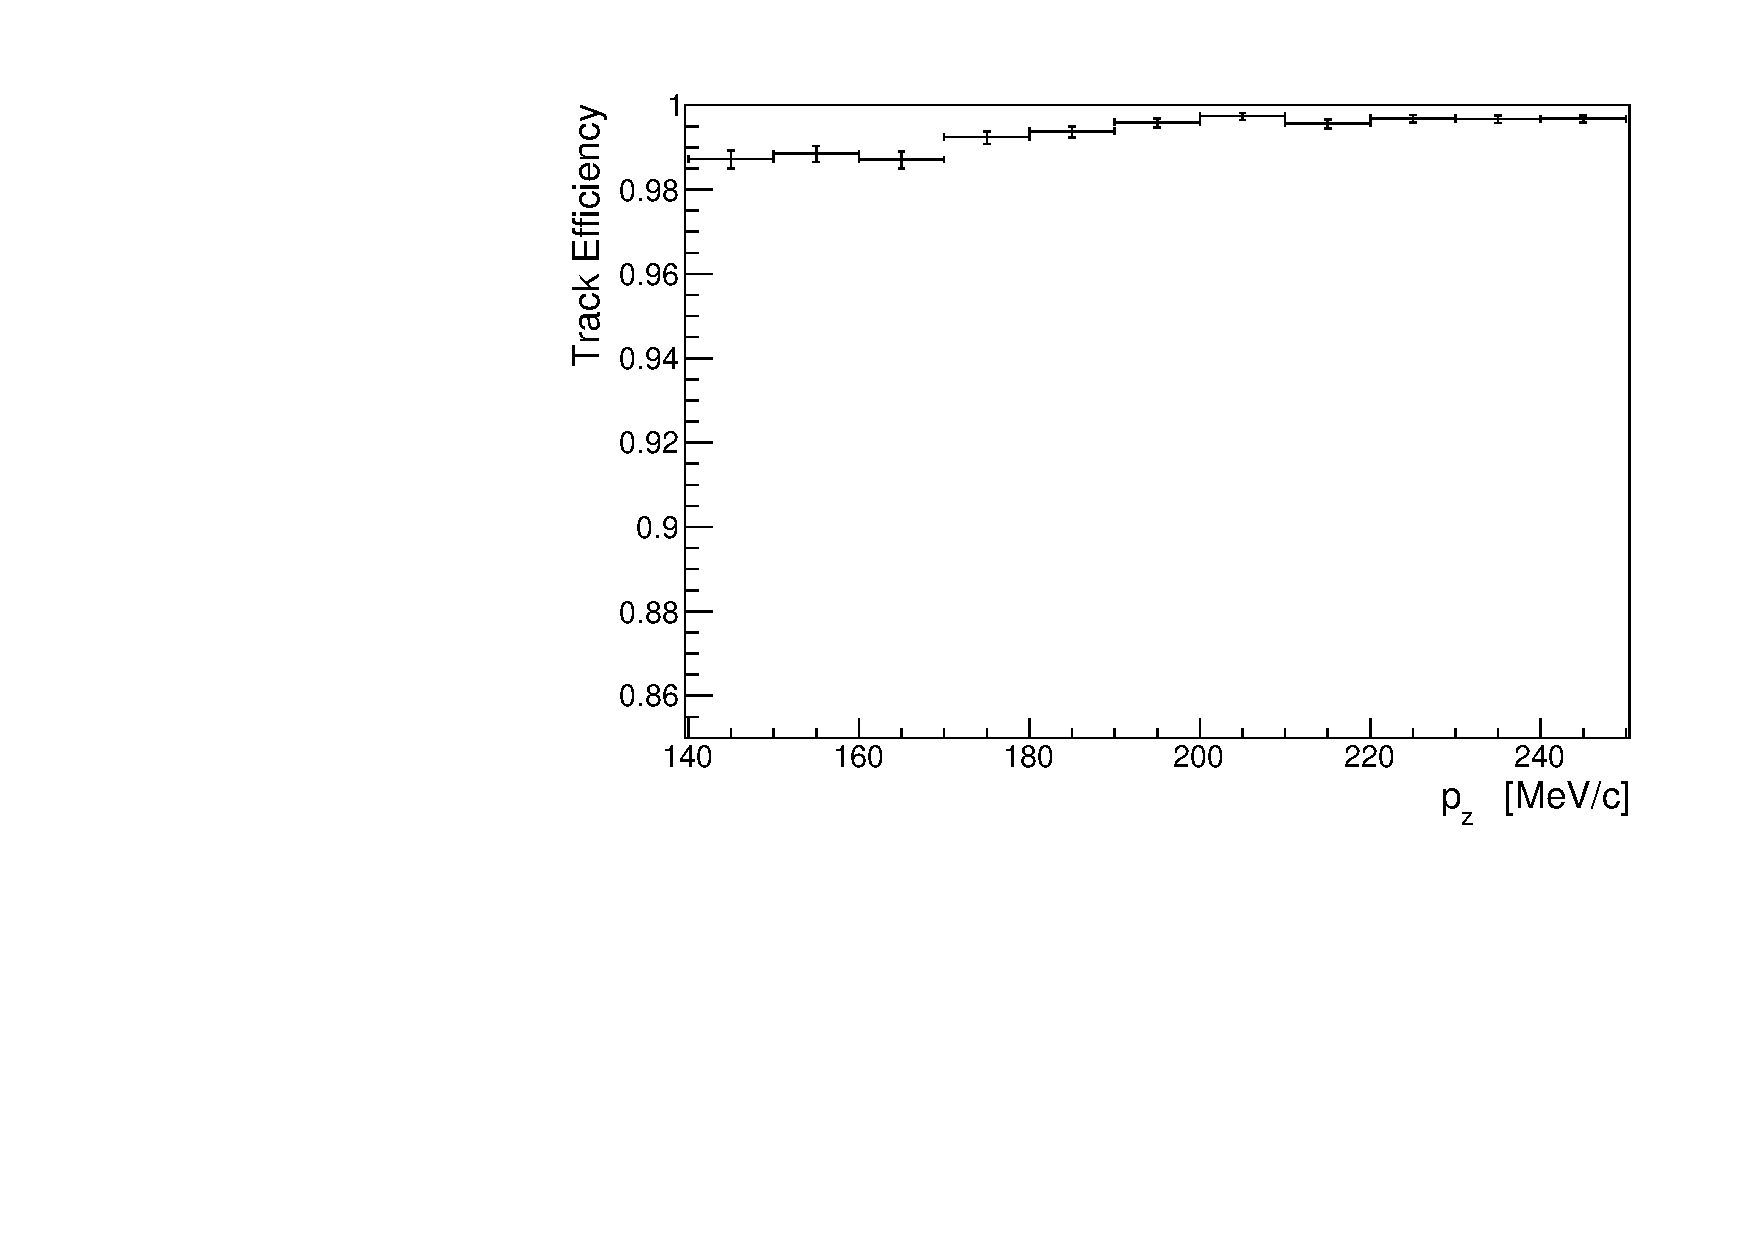
\includegraphics[width=0.45\textwidth, angle=0]{08-Performance/upstream_pz_track_efficiency.pdf}
    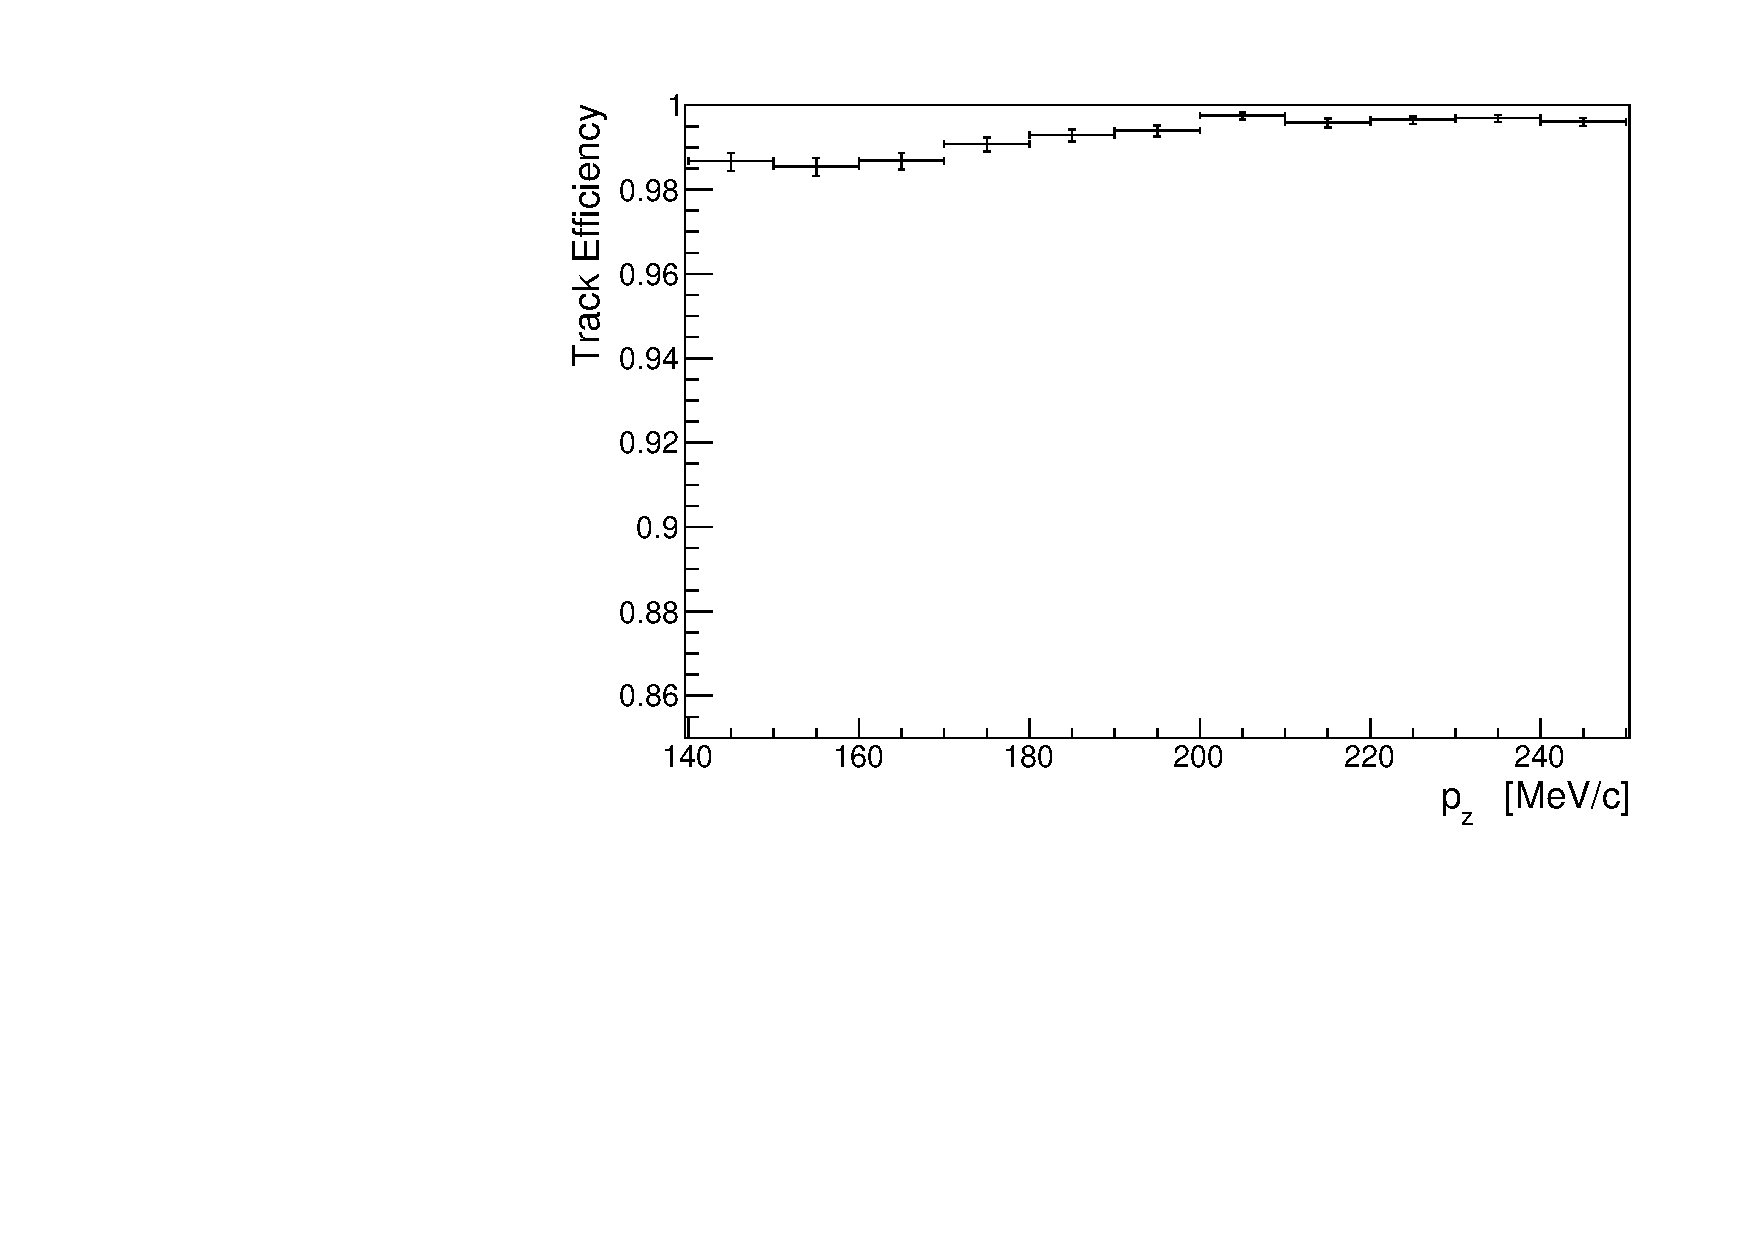
\includegraphics[width=0.45\textwidth, angle=0]{08-Performance/downstream_pz_track_efficiency.pdf}\\
    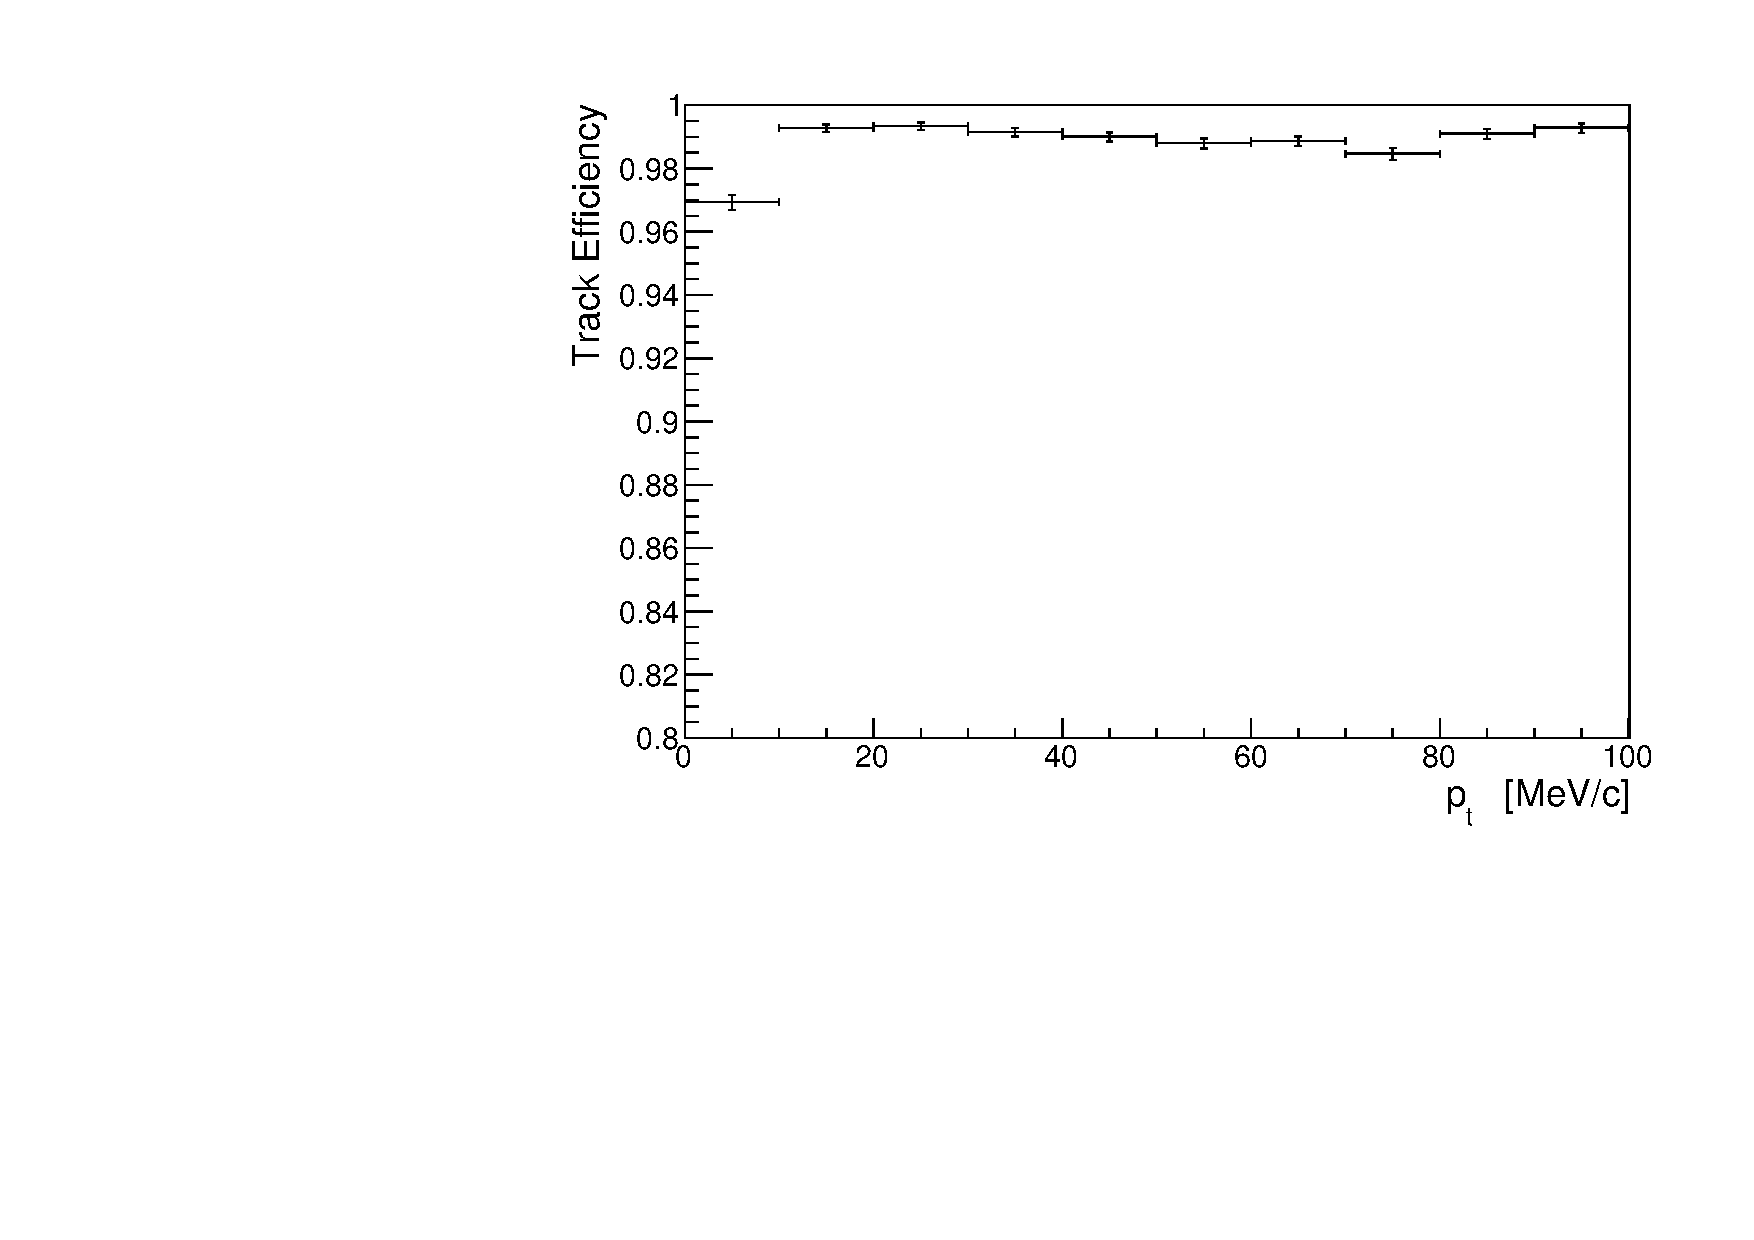
\includegraphics[width=0.45\textwidth, angle=0]{08-Performance/upstream_pt_track_efficiency.pdf}
    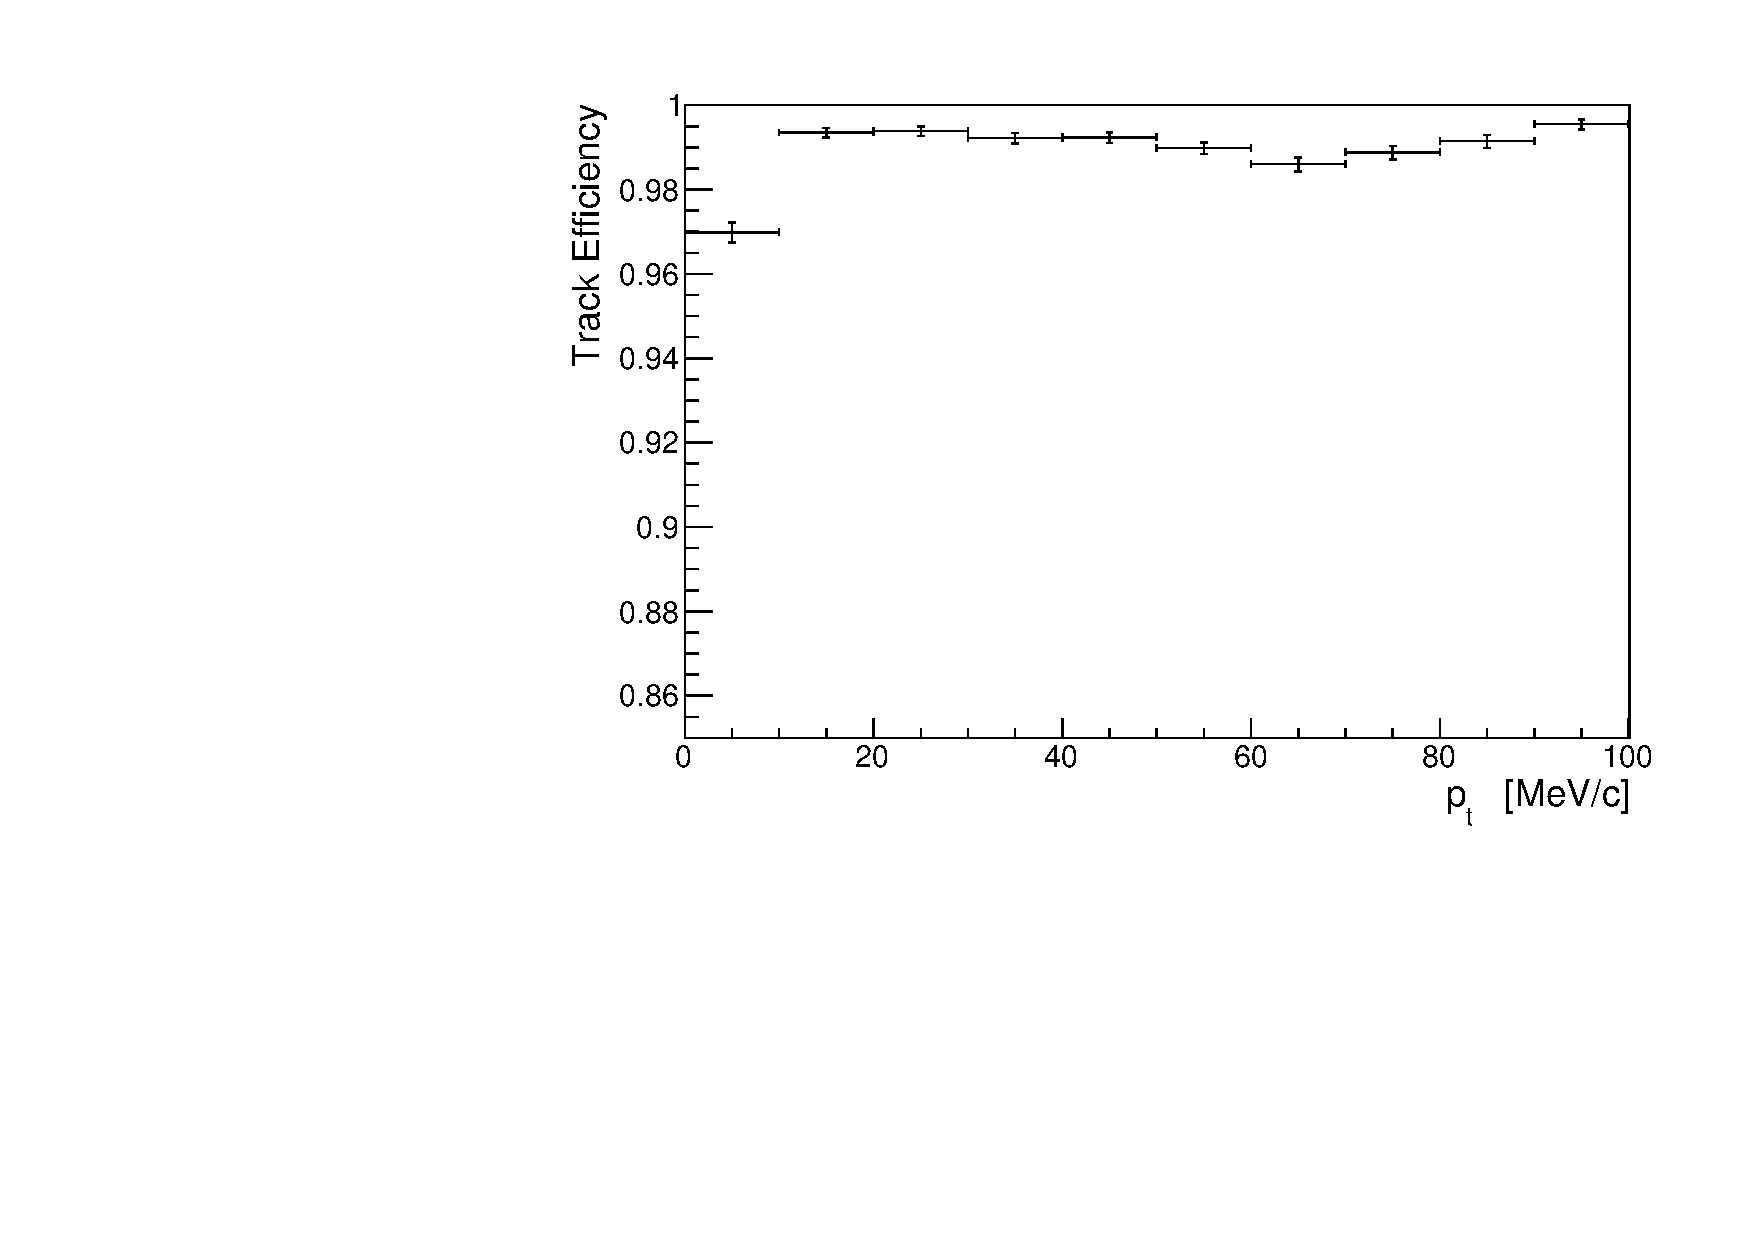
\includegraphics[width=0.45\textwidth, angle=0]{08-Performance/downstream_pt_track_efficiency.pdf}
    \caption{\label{fig:track_efficiency} The efficiency of reconstructing tracks in the upstream (left) and downstream (right) trackers as a function of the simulated longitudinal (top) and transverse (bottom) momentum.}
  \end{figure}

  Once the the Monte Carlo tracks have been identified, the expected number of trackpoints can be calculated by examining the number of tracker planes that the simulated track crossed. Comparing the number of trackpoints in each reconstructed track to the expected number for each simulated track permits the efficiency of finding the correct number of trackpoints to be calculated. Figure~\ref{fig:tp_efficiency} shows the trackpoint finding efficiency as a function of longitudinal and transverse momenta.

  \begin{figure}[p]
    \centering
    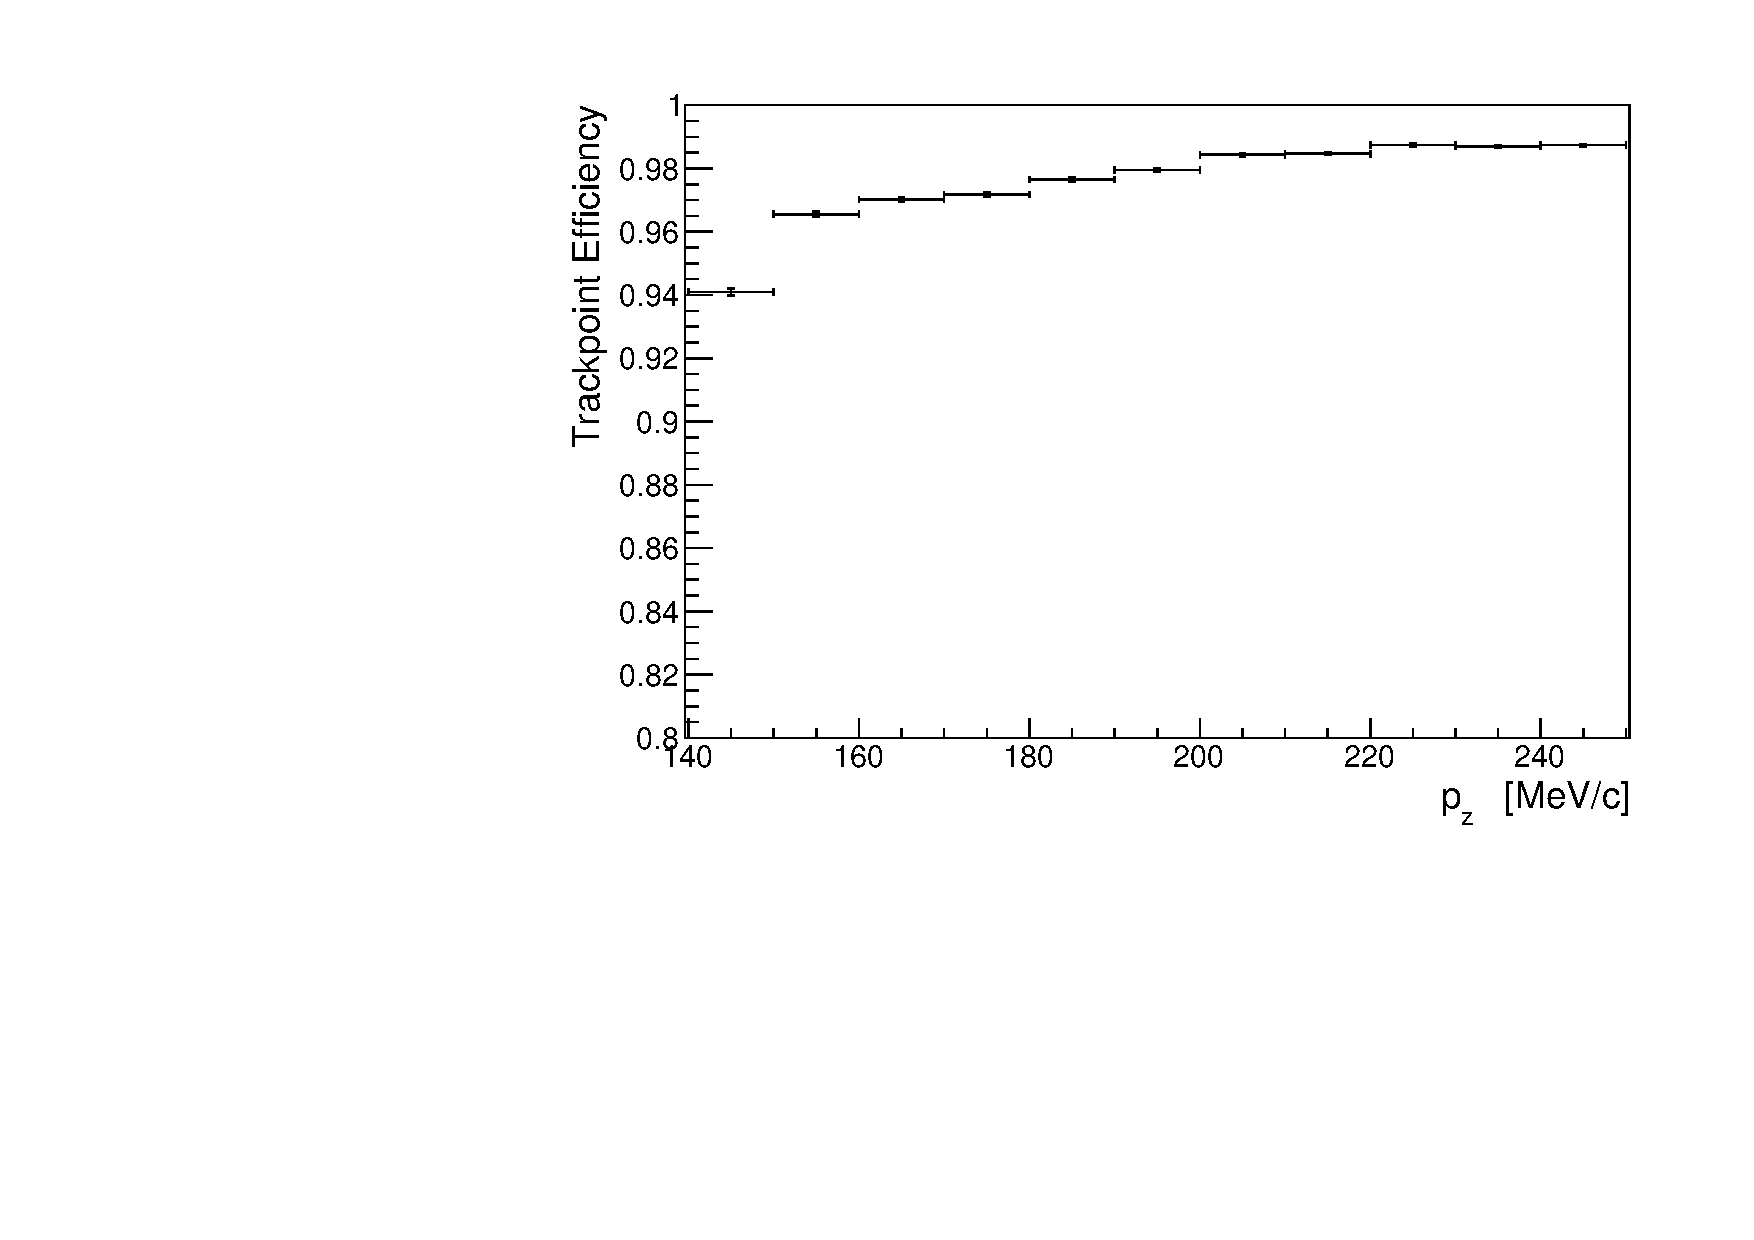
\includegraphics[width=0.45\textwidth, angle=0]{08-Performance/upstream_pz_tp_efficiency.pdf}
    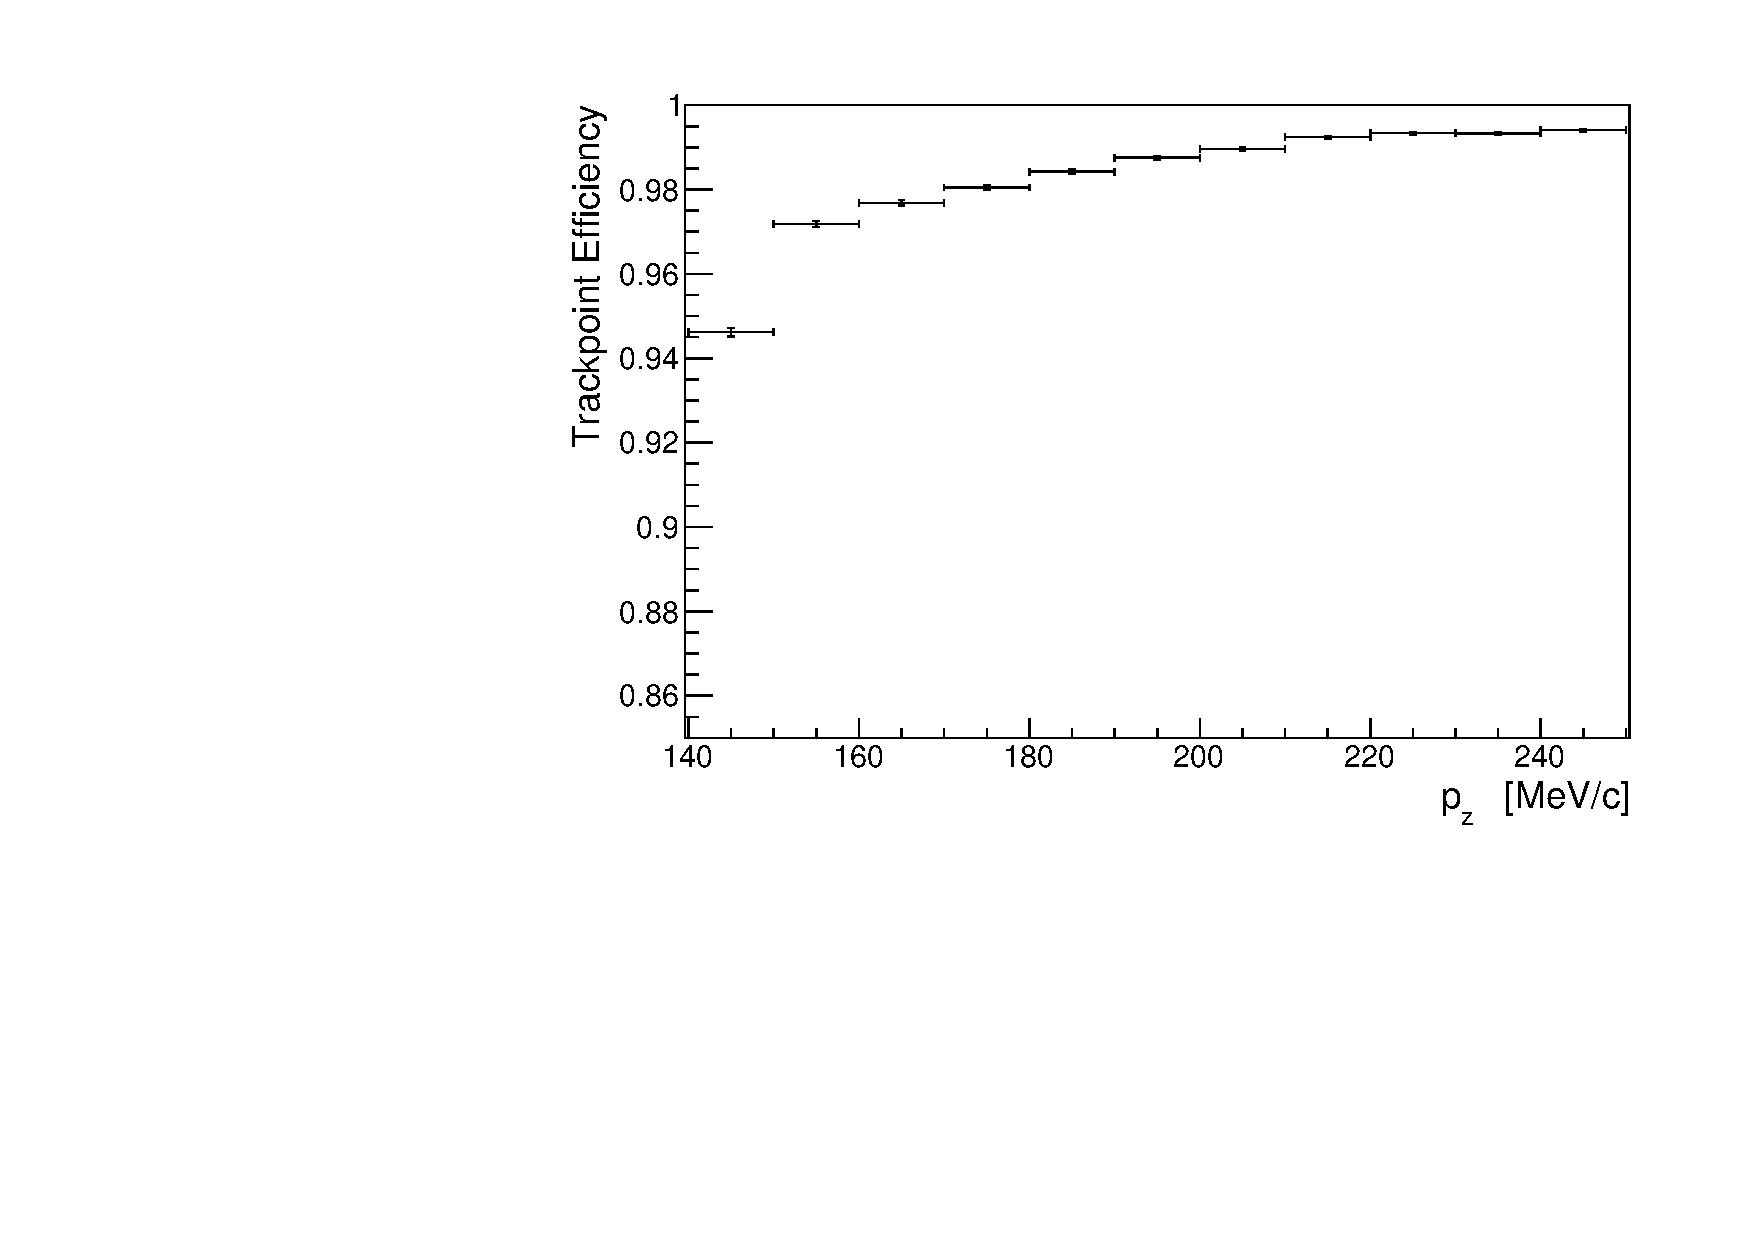
\includegraphics[width=0.45\textwidth, angle=0]{08-Performance/downstream_pz_tp_efficiency.pdf}\\
    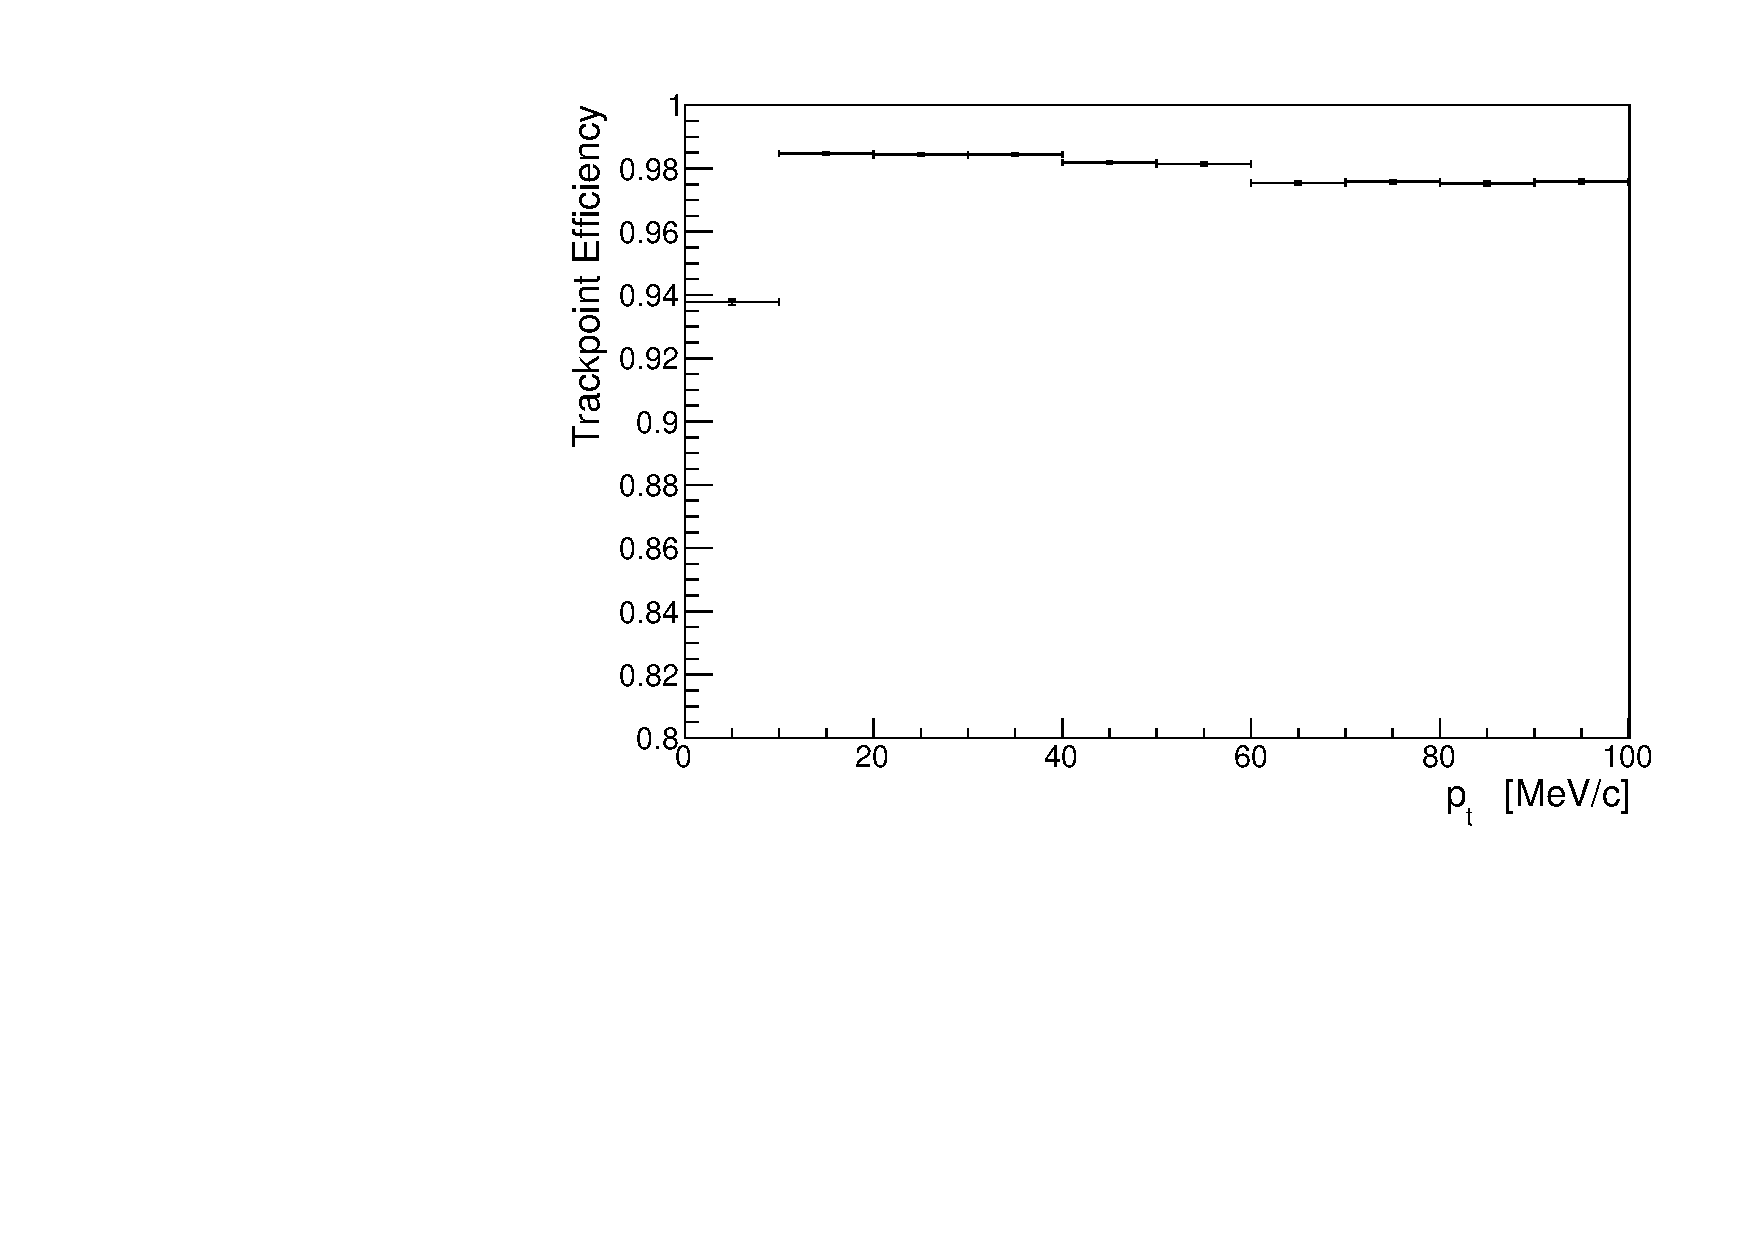
\includegraphics[width=0.45\textwidth, angle=0]{08-Performance/upstream_pt_tp_efficiency.pdf}
    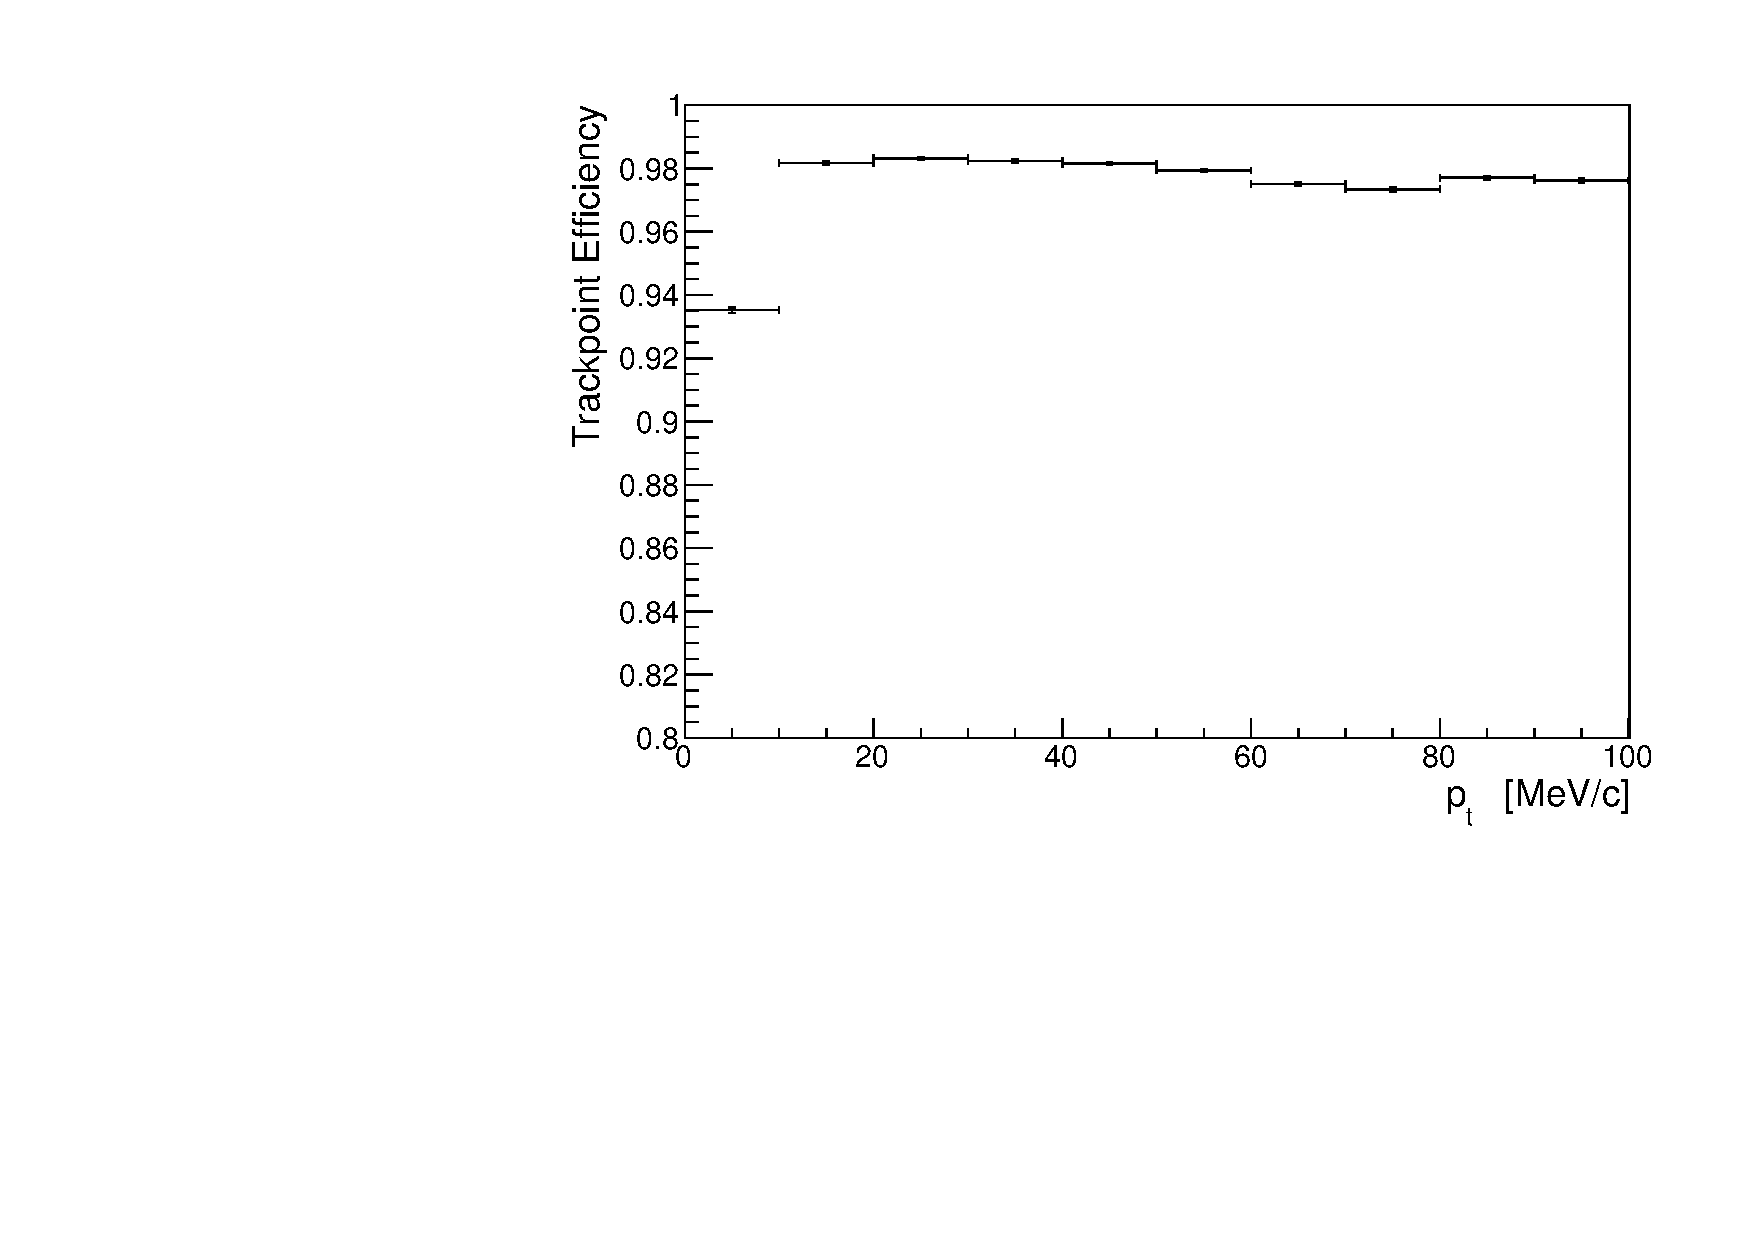
\includegraphics[width=0.45\textwidth, angle=0]{08-Performance/downstream_pt_tp_efficiency.pdf}
    \caption{\label{fig:tp_efficiency} The efficiency of reconstructing trackpoints in the upstream (left) and downstream (right) trackers as a function of the simulated longitudinal (top) and transverse (bottom) momentum.}
  \end{figure}


  \subsection{Reconstruction Resolution}
  \label{sec:performance:resolutions}
  
  Position residuals are shown in figures~\ref{fig:XResidKalman} and \ref{fig:YResidKalman}, and the momentum residuals in figures~\ref{fig:PtResidKalman} and \ref{fig:PzResidKalman}.  The position reconstruction can be seen to agree with the Monte Carlo truth to high precision in both the upstream and downstream trackers. The momentum residuals currently display some systematic effect which is due to uncertainty in the determination of energy loss within the tracker and the accuracy of the pattern recognition parameters.

  The position residuals are consistent with the expected measurement resolutions for a combined fit and the absolute spread is very close to the width of a channel (1.497~mm). The transverse momentum resolution is consistent across the range of the sensitive phase space at $\sim$1.2~MeV/c in both trackers. The longitudinal momentum, an intrinsically more difficult measurement for the tracker, still retains an acceptable spread of ${\sim4}$~MeV/c in both trackers. There is however a small ($<0.1$~MeV/c) systematic effect, visible in the momentum distributions.

  In order to produce these plots, a requirement that there was a cluster within the reference plane was applied. Due to the effects of Multiple Coulomb Scattering, on rare occasions a single hard scatter can cause pattern recognition to miss a single spacepoint at the reference plane, hence creating a tail that will adversely affect the distributions. As we are concerned with the resolution following a successful pattern recognition stage, these events were removed.
  
  
  The track fit assumes a simple model of energy loss based on the mean thickness of materials used in the tracker construction, however the effects of glues and resins, in addition to the non-uniform densities of the materials are not considered. This results in systematic underestimate for the energy lost at each tracker plane and a small sytematic bias during the pattern recognition stage, which doesn't attempt to model these effects. Due to the high-granularity of the position information utilised by the fit, the position reconstruction is much less sensitive to any discrepancies in momentum. Figure~\ref{fig:pBiasKalman} shows the mean deviation in total reconstructed momentum across the typical momentum acceptance of the trackers.

  Trends in transverse and longitudinal momentum resolution as a function of transverse momentum are shown in figures~\ref{fig:PtPtResolKalman} and \ref{fig:PtPzResolKalman}. A consistently uniform distribution is found in the transverse momentum as expected, with the predominant issue found in the longitudinal reconstruction of low-$p_t$ tracks. This effect, when coupled with variations in efficiency will yield some systematic concerns in the reconstruction of statistical quantities such as emittance. Studies of these systematic biases are currently under way.

  \begin{figure}[hb]
    \begin{center}
      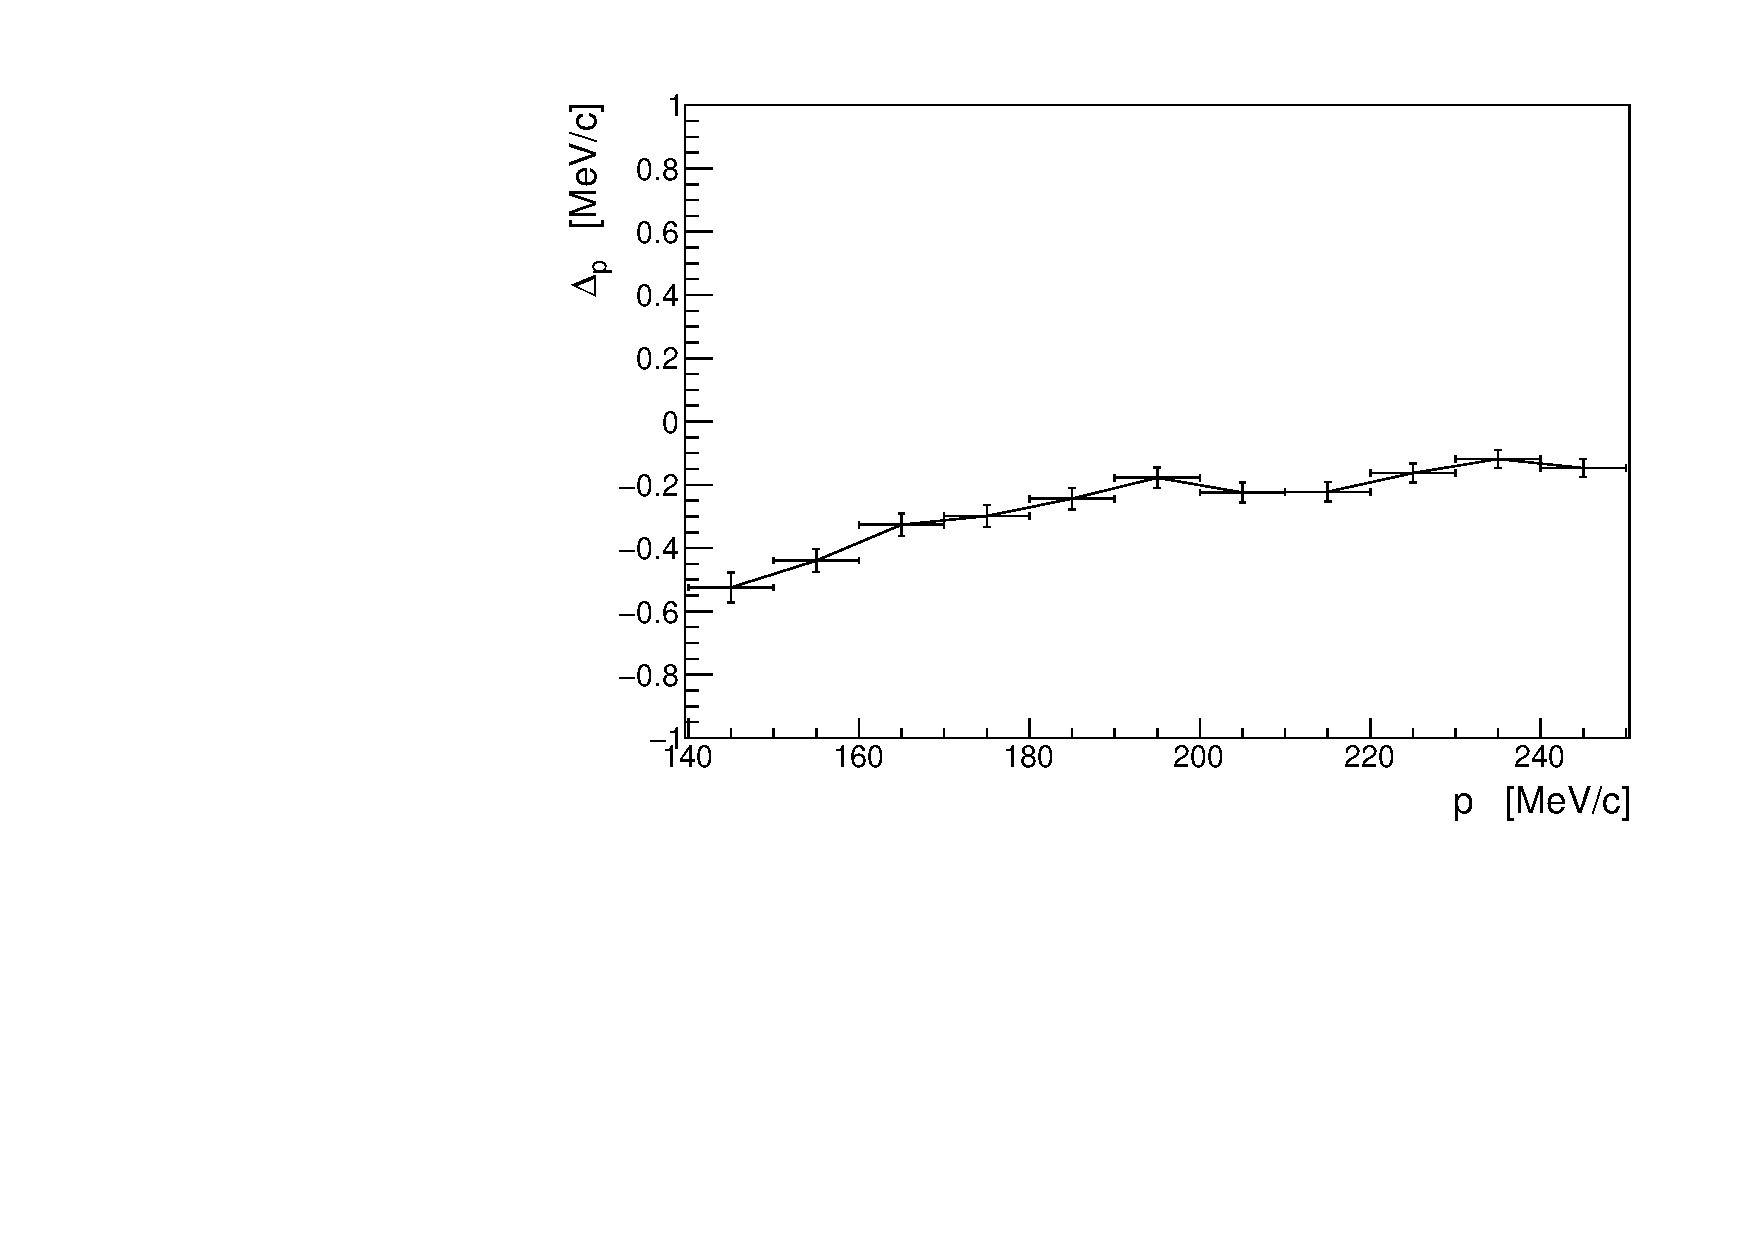
\includegraphics[width=0.49\textwidth, angle=0]{08-Performance/upstream_p_bias_p.pdf}
      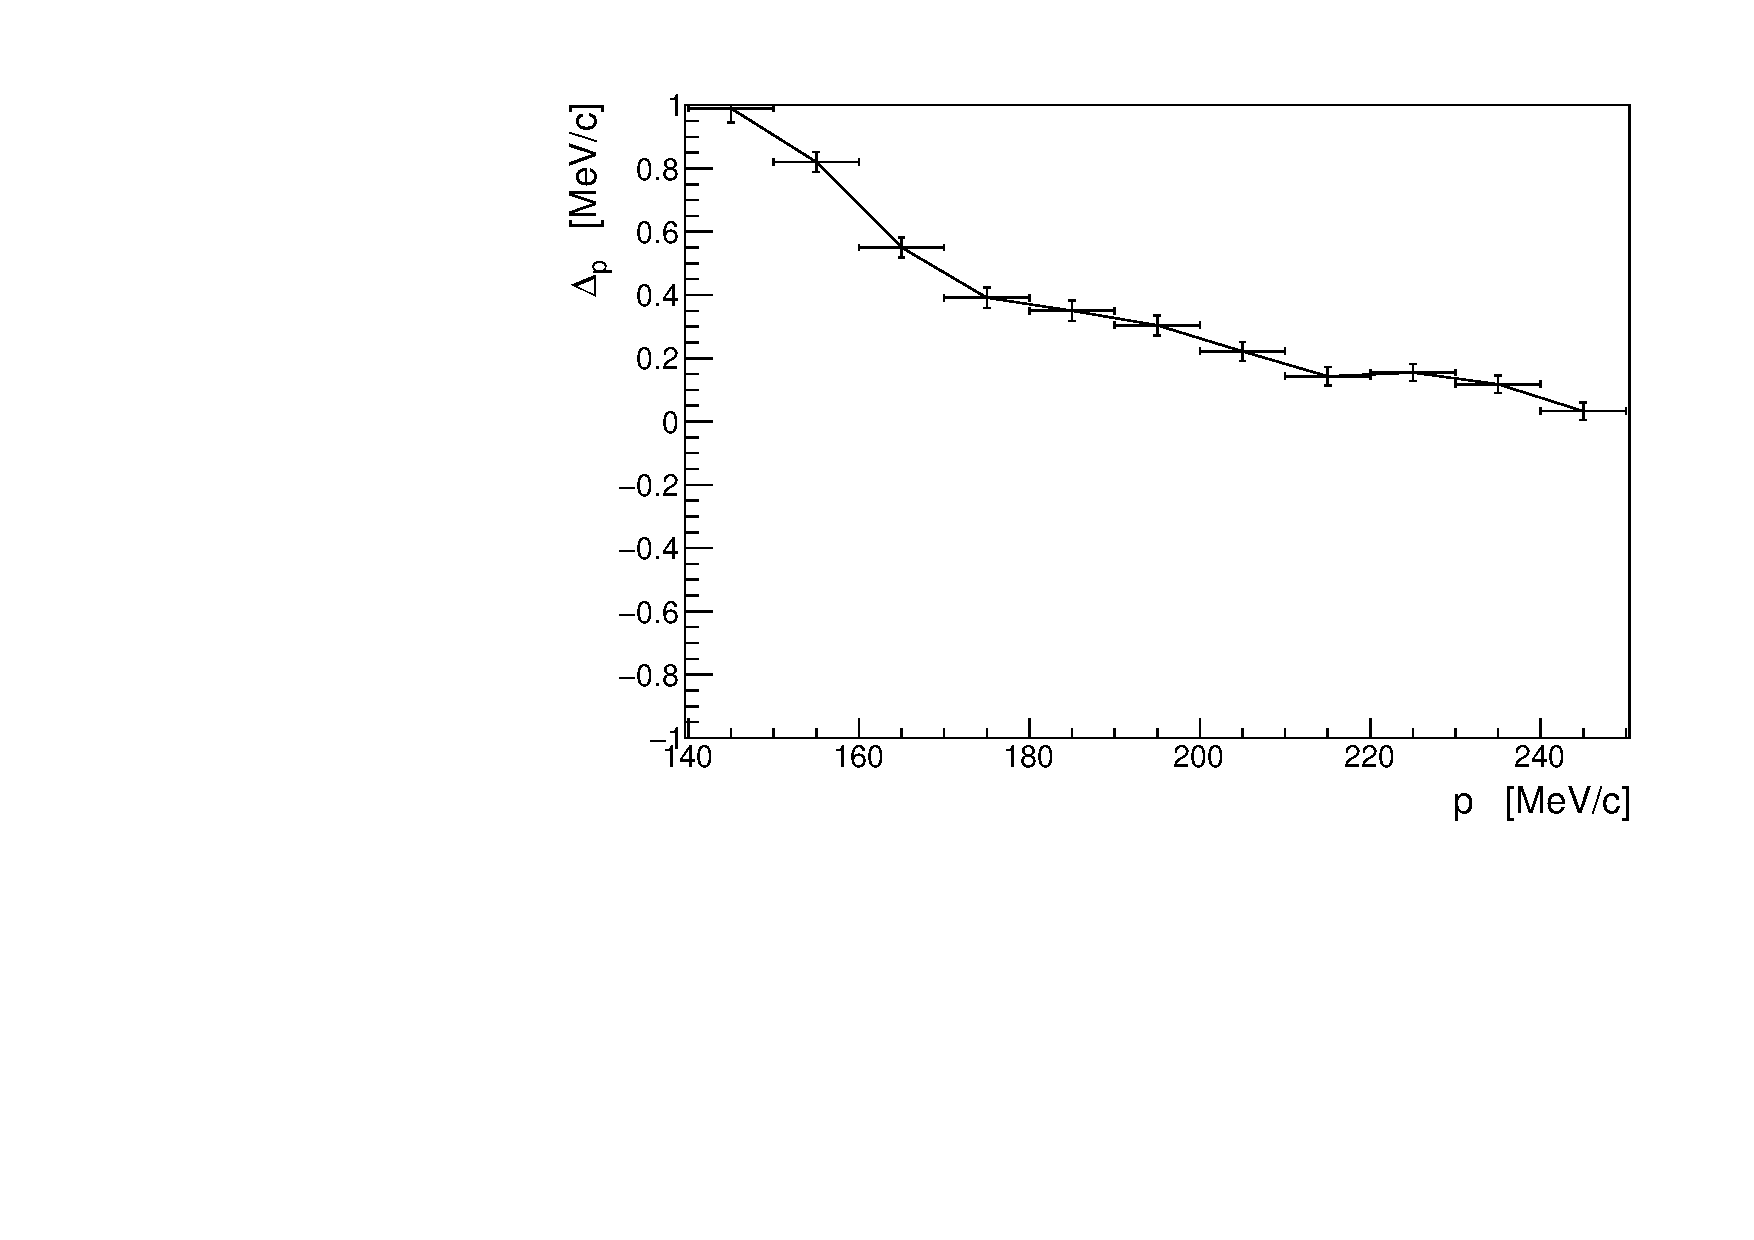
\includegraphics[width=0.49\textwidth, angle=0]{08-Performance/downstream_p_bias_p.pdf}
      \caption{\label{fig:pBiasKalman} The mean residual between the final track fit total momentum and the true track momentum, evaluated at the reference plane.}
    \end{center}
  \end{figure}

  \begin{figure}[p]
    \begin{center}
      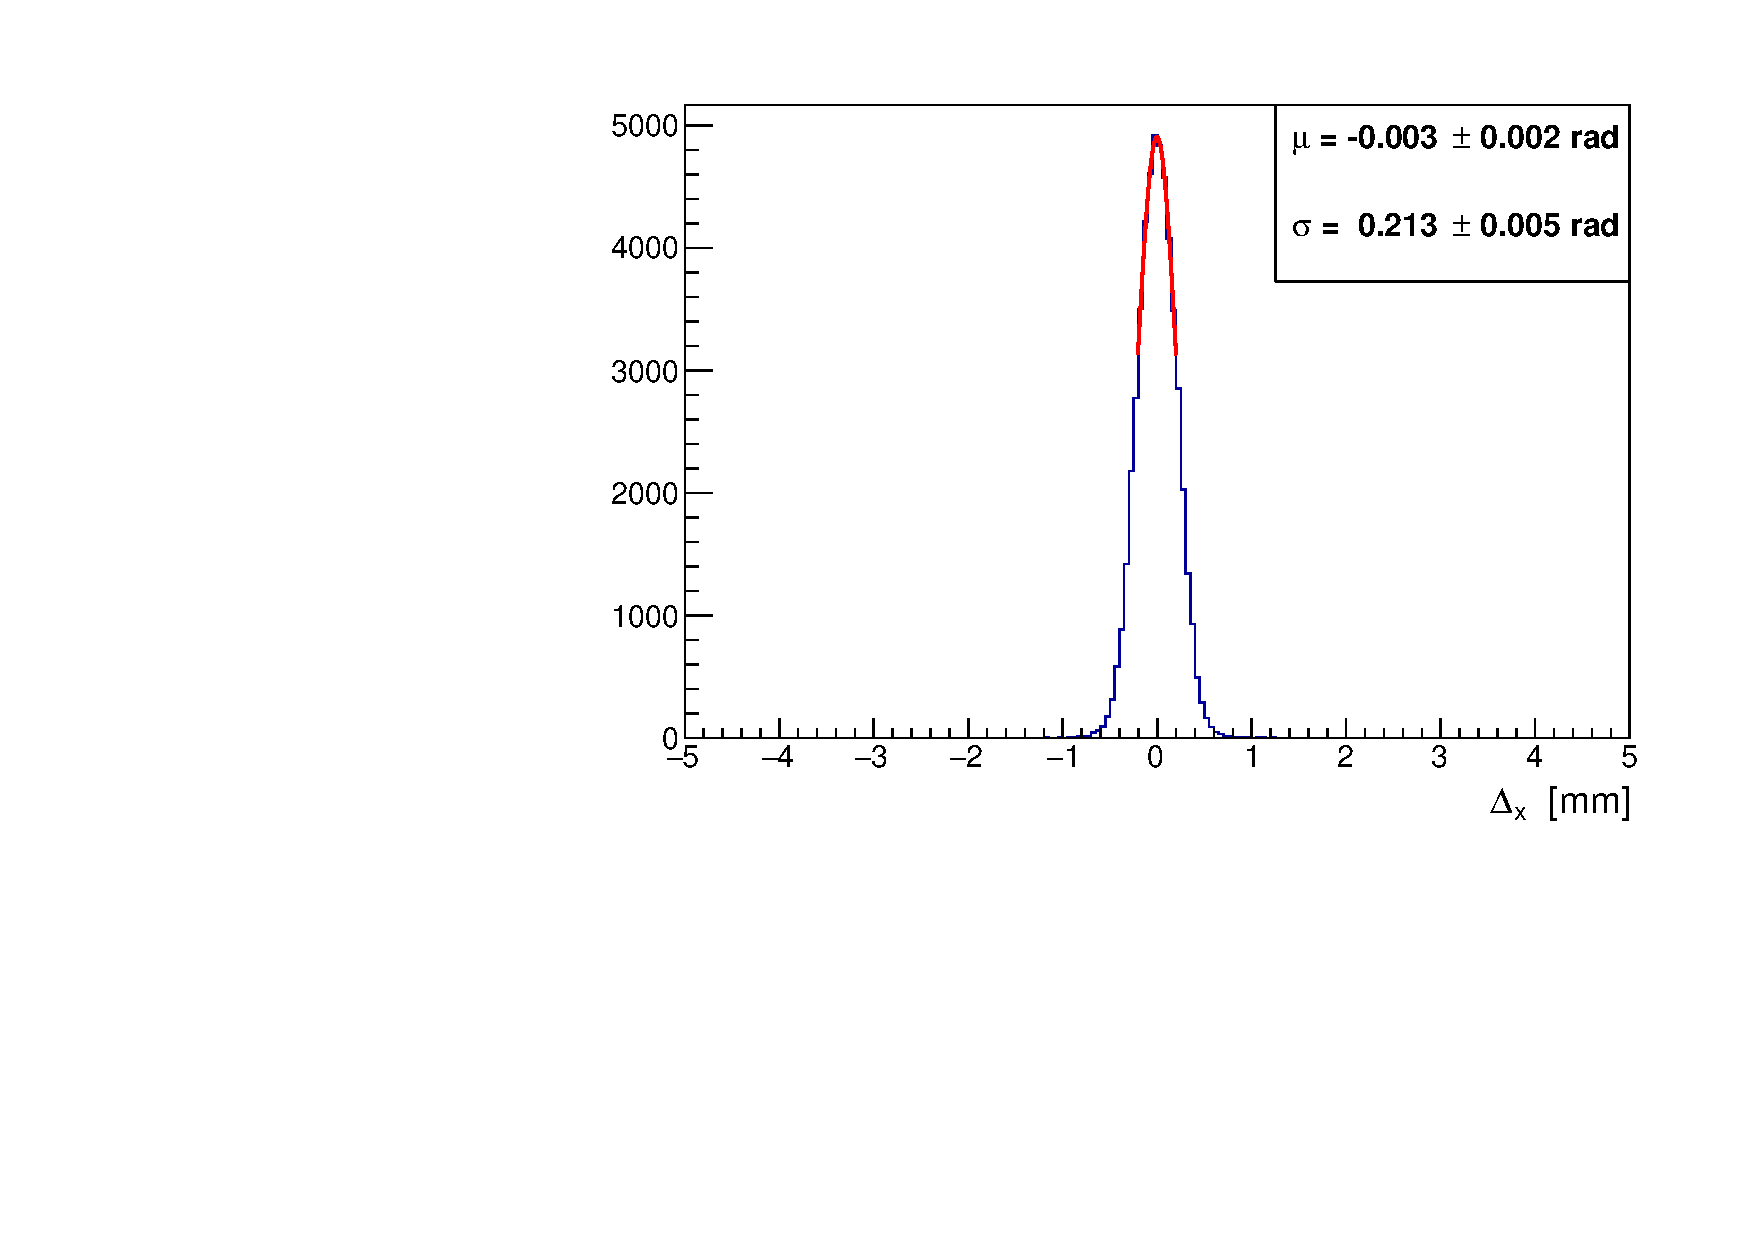
\includegraphics[width=0.49\textwidth, angle=0]{08-Performance/upstream_x_residual.pdf}
      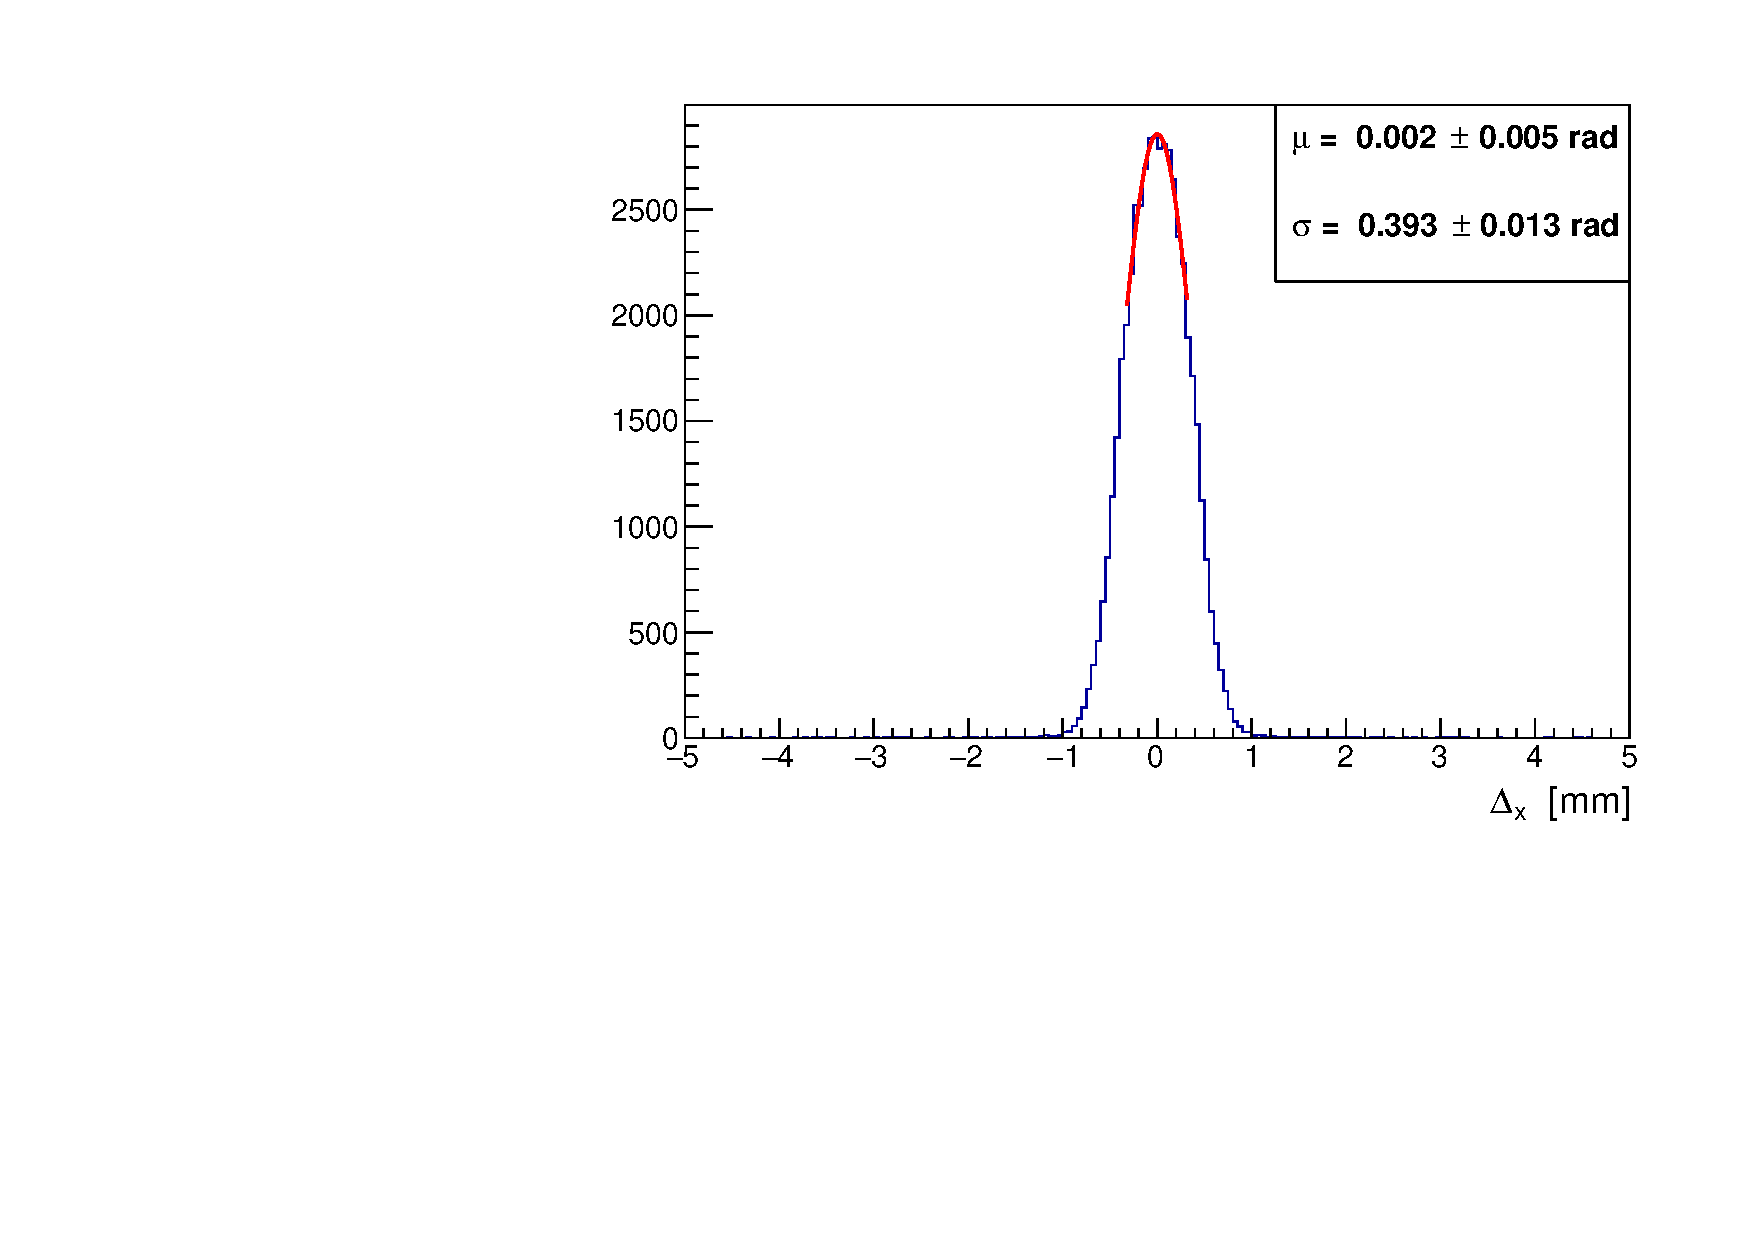
\includegraphics[width=0.49\textwidth, angle=0]{08-Performance/downstream_x_residual.pdf}
      \caption{\label{fig:XResidKalman} The $x$ residuals of the upstream (left) and downstream (right) trackers.}
    \end{center}
  \end{figure}
  
    \begin{figure}[p]
    \begin{center}
      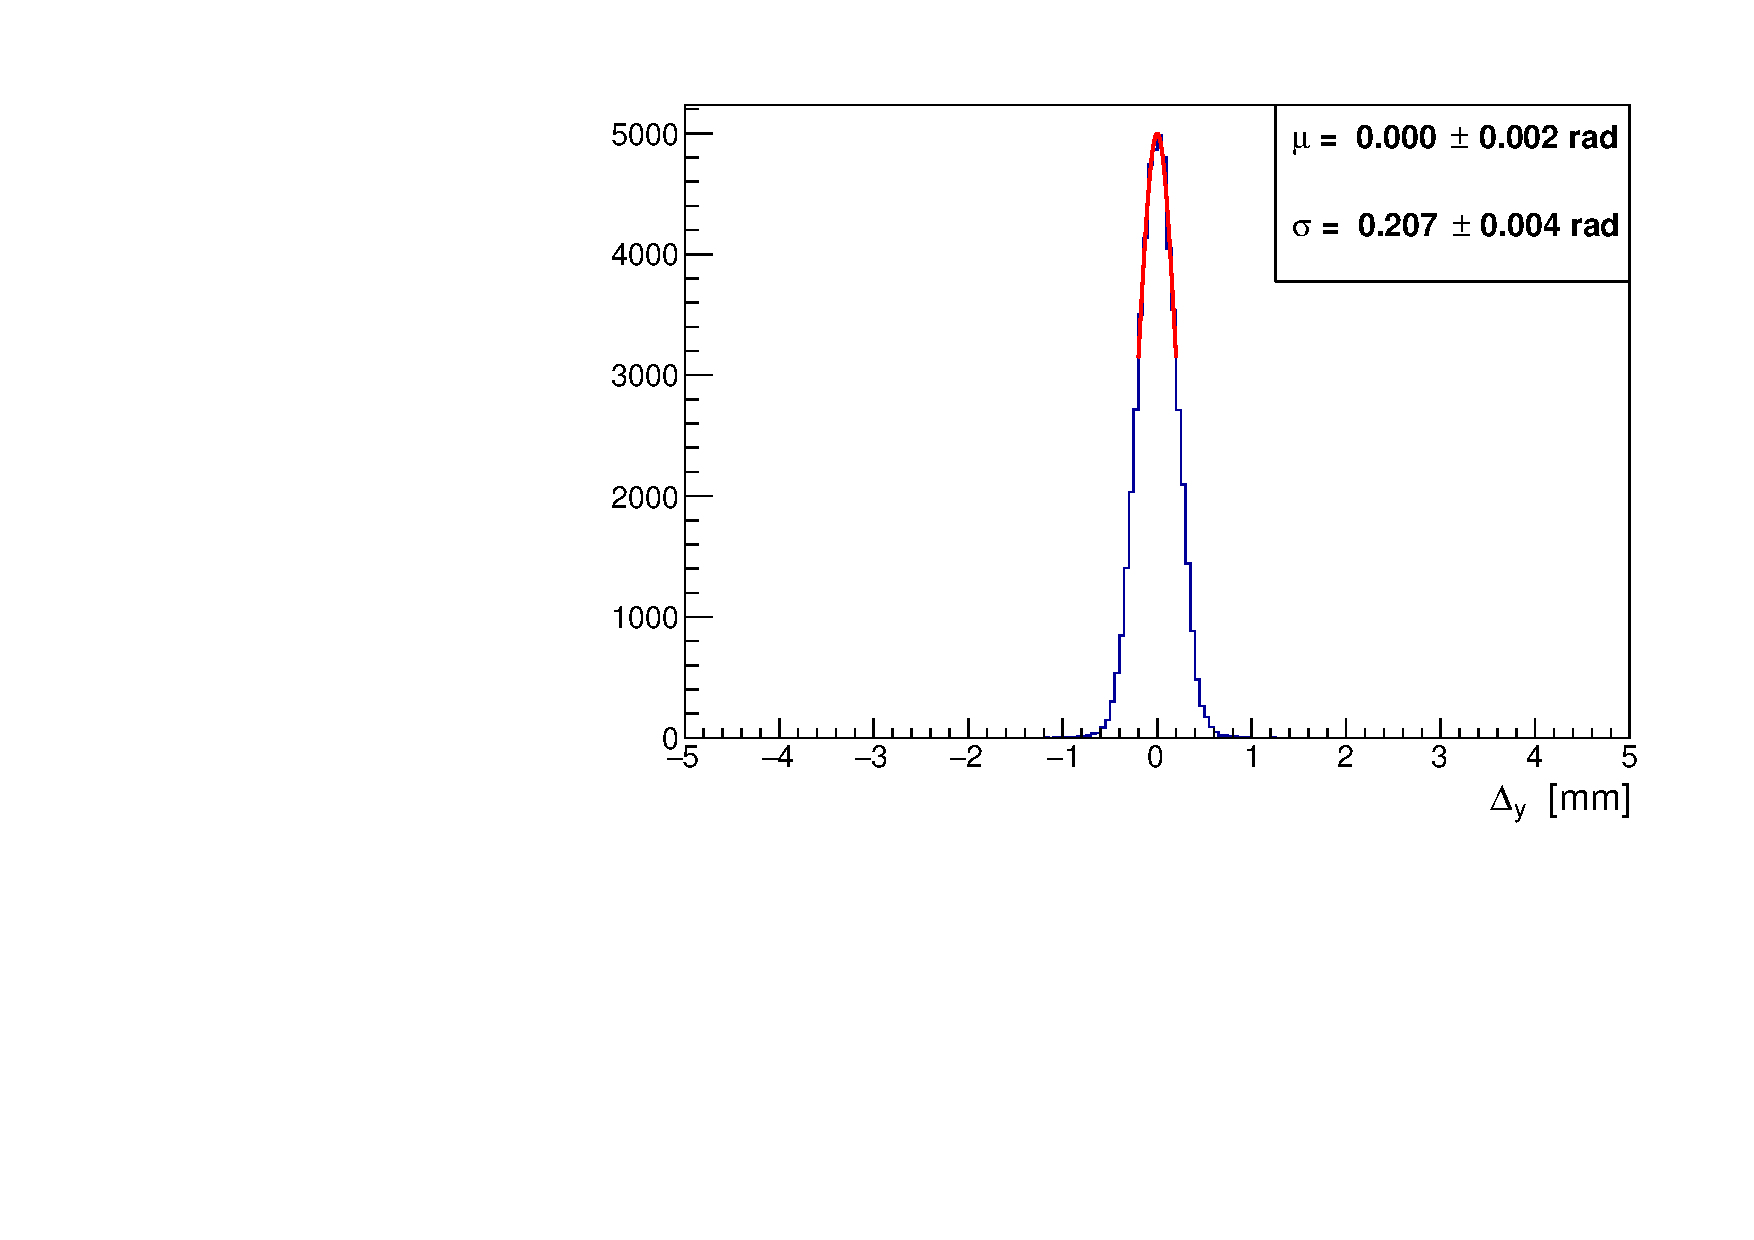
\includegraphics[width=0.49\textwidth, angle=0]{08-Performance/upstream_y_residual.pdf}
      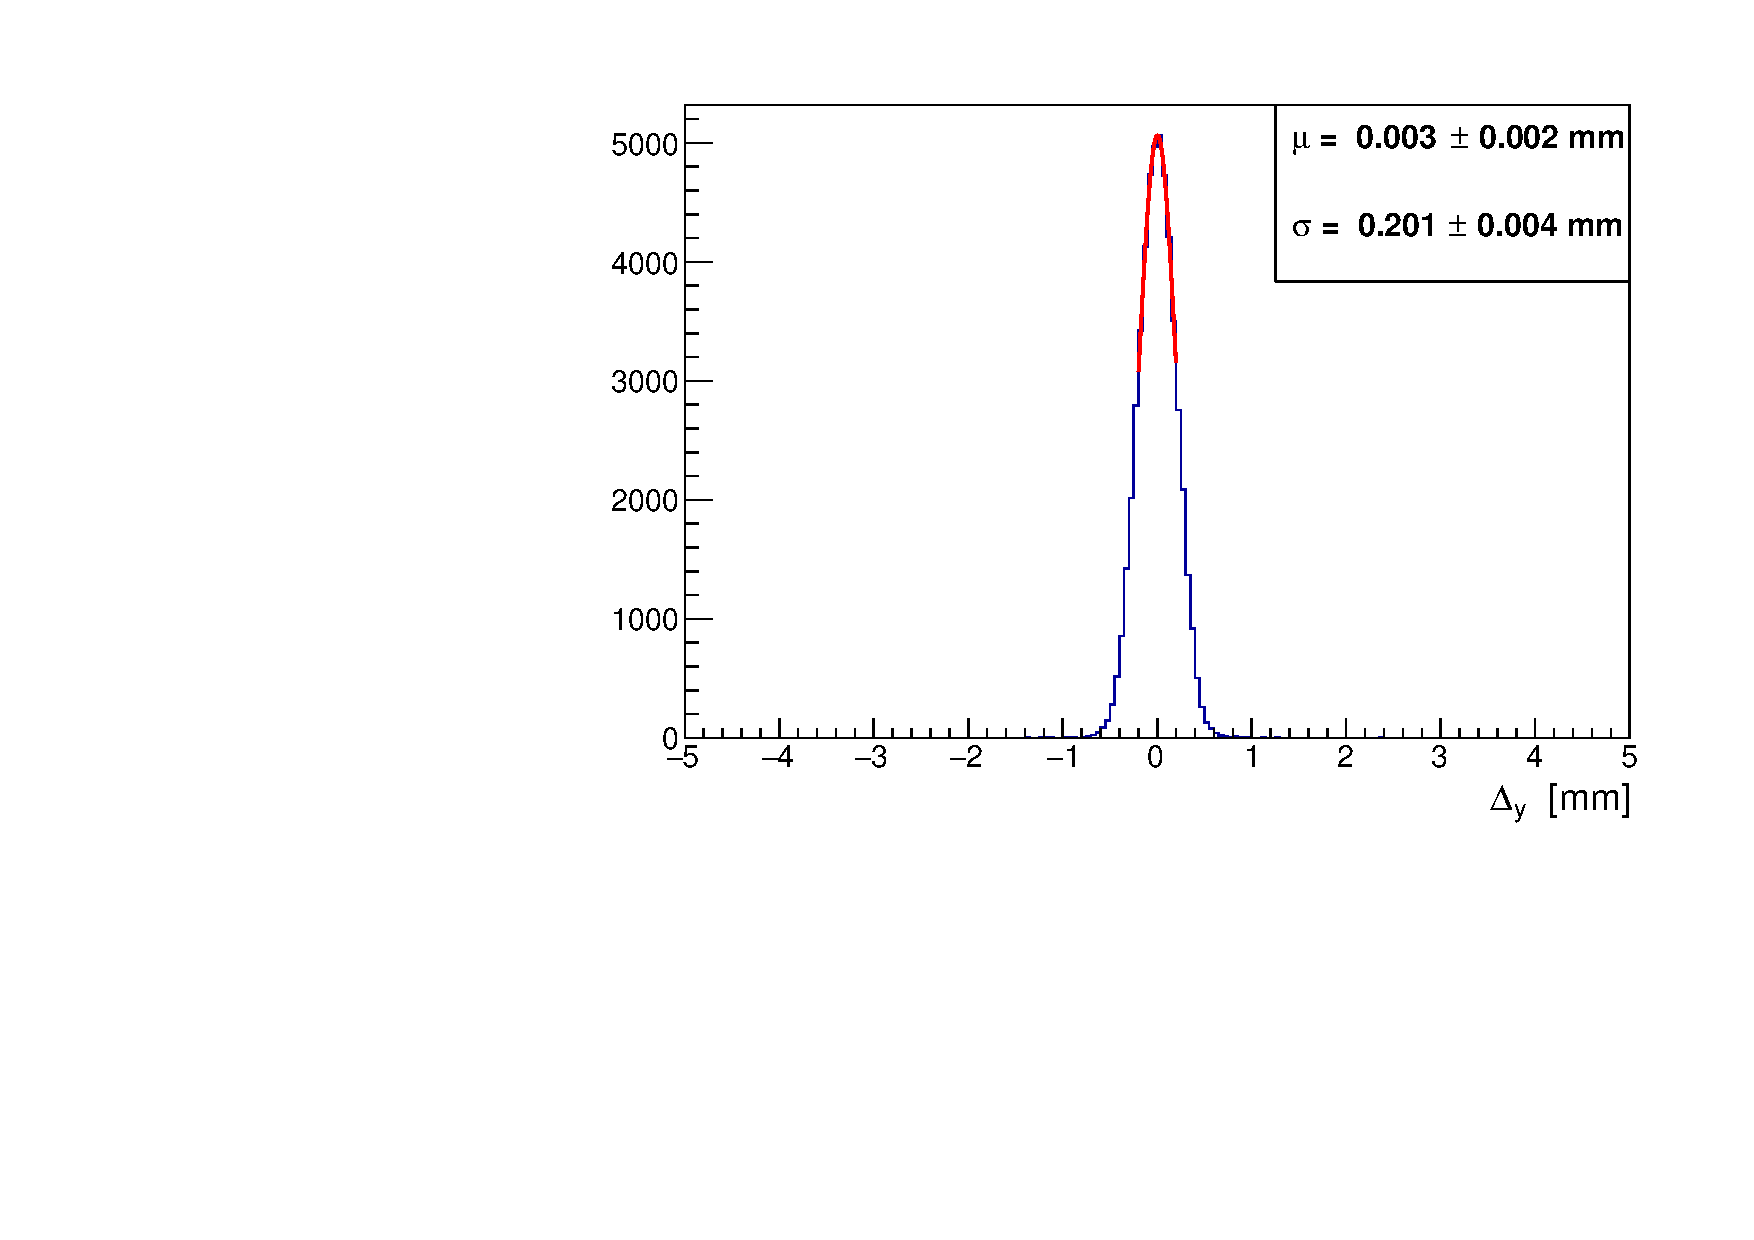
\includegraphics[width=0.49\textwidth, angle=0]{08-Performance/downstream_y_residual.pdf}
      \caption{\label{fig:YResidKalman} The $y$ residuals of the upstream (left) and downstream (right) trackers.}
    \end{center}
  \end{figure}
  
  
  \begin{figure}[p]
    \begin{center}
      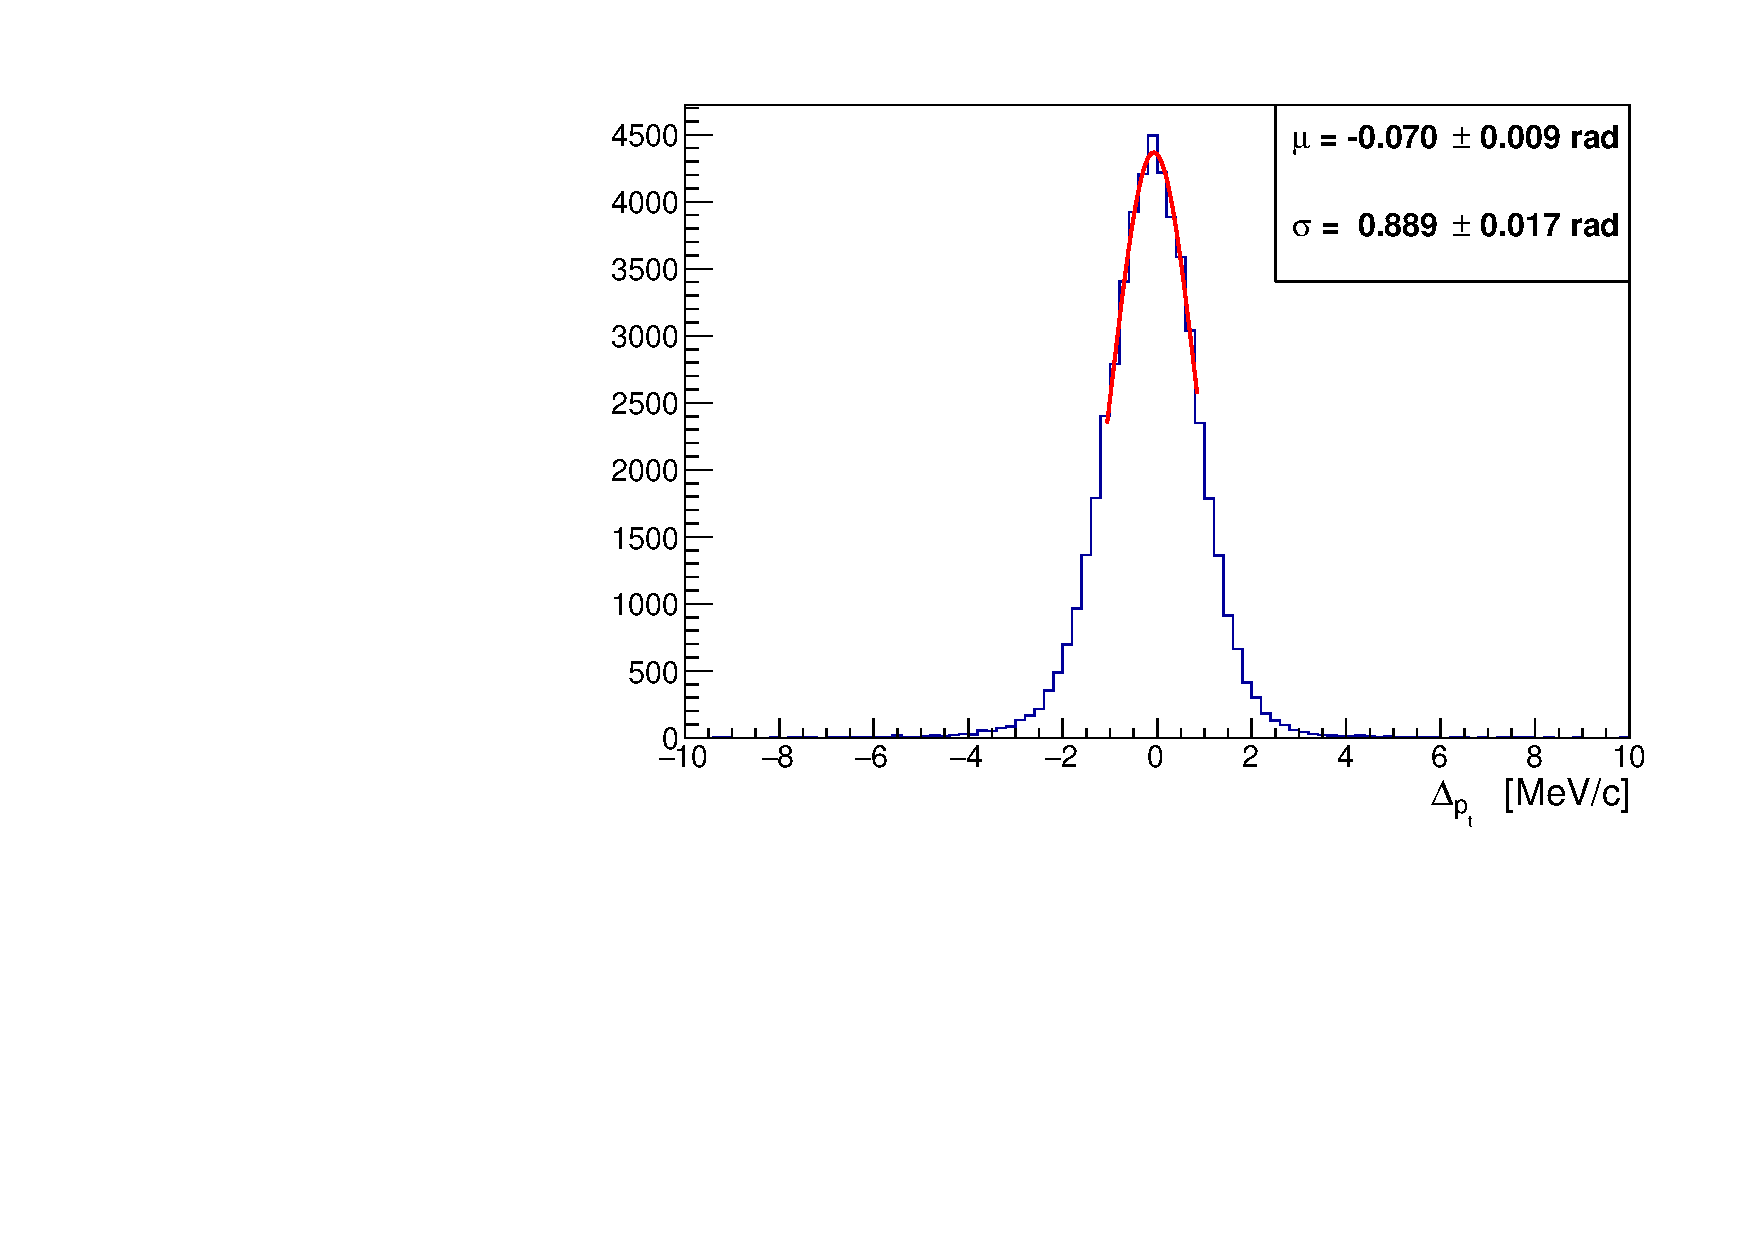
\includegraphics[width=0.49\textwidth, angle=0]{08-Performance/upstream_pt_residual.pdf}
      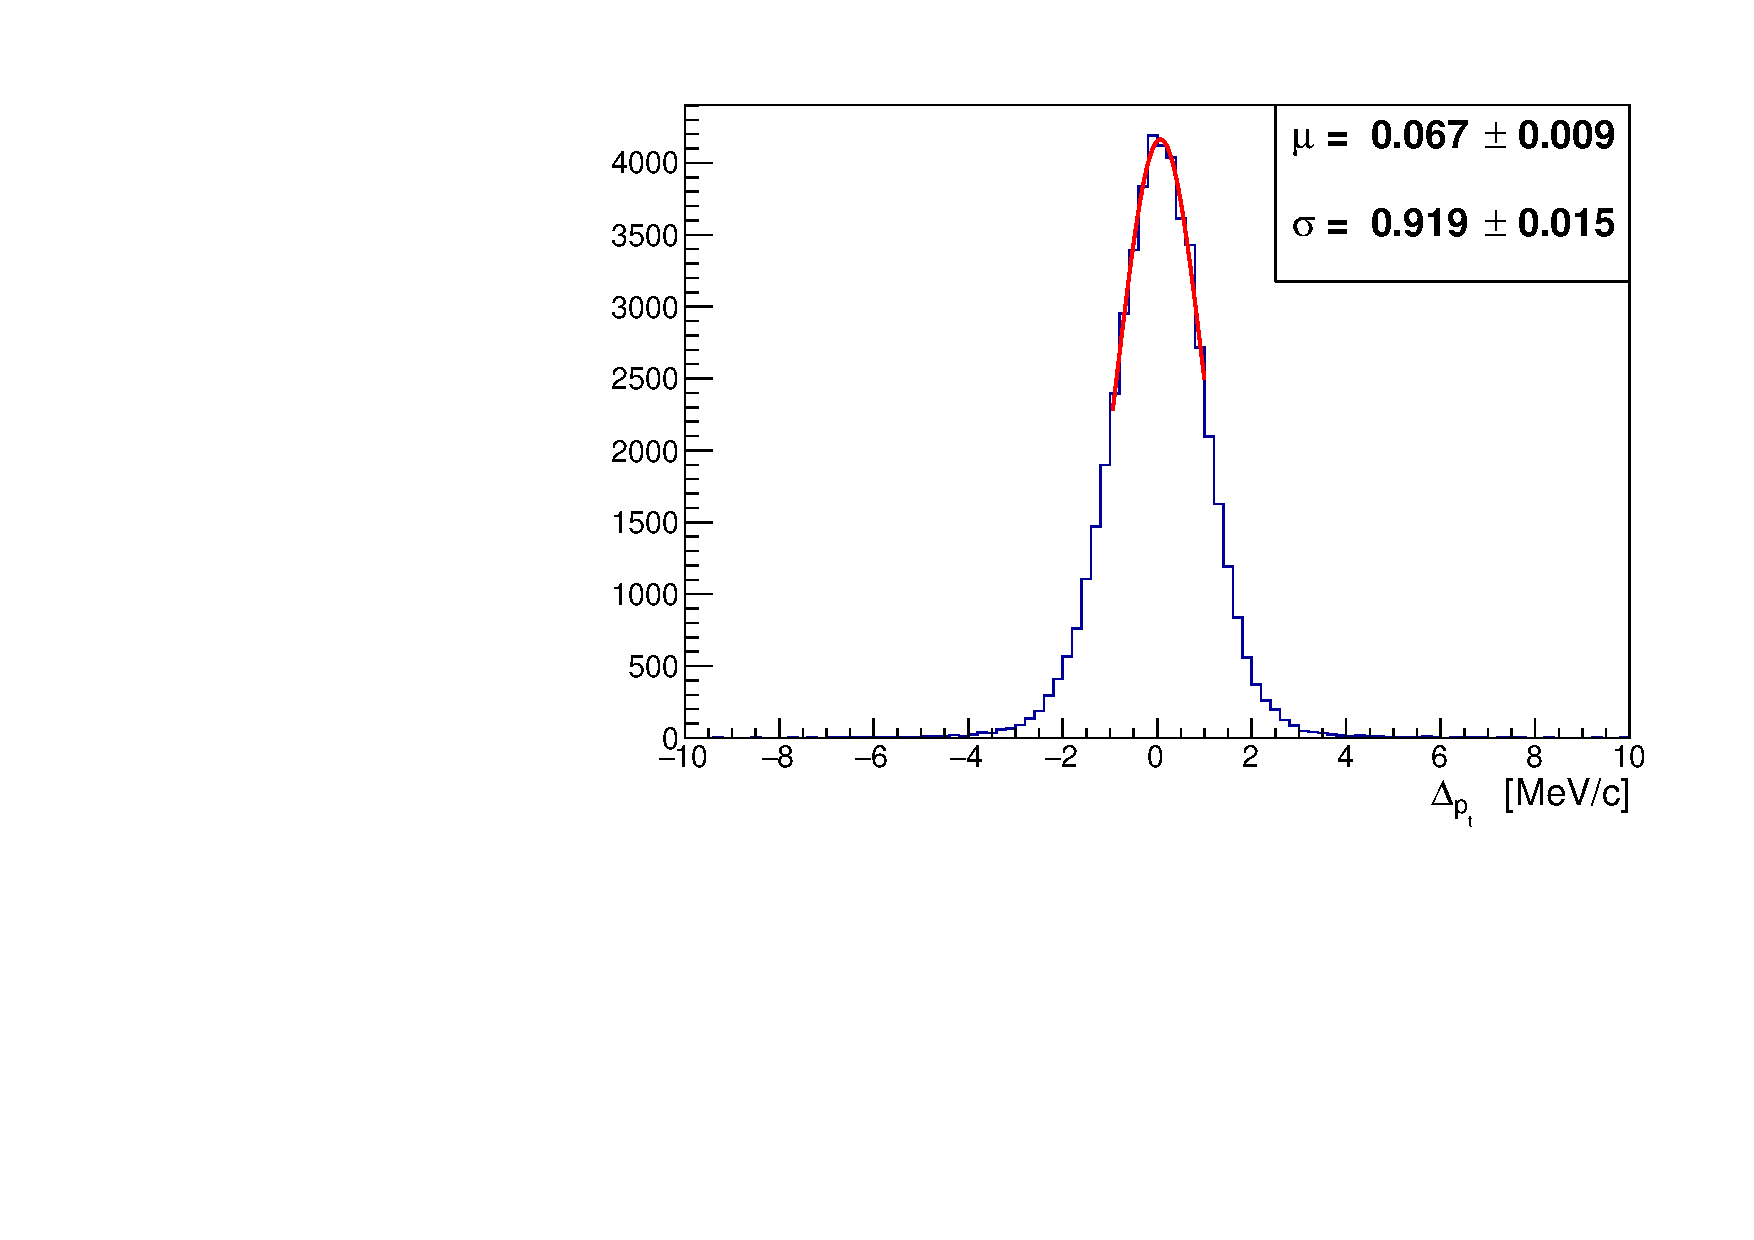
\includegraphics[width=0.49\textwidth, angle=0]{08-Performance/downstream_pt_residual.pdf}
      \caption{\label{fig:PtResidKalman} The $p_{t}$ residuals of the upstream (left) and downstream (right) trackers.}
    \end{center}
  \end{figure}
  
   \begin{figure}[p]
    \begin{center}
      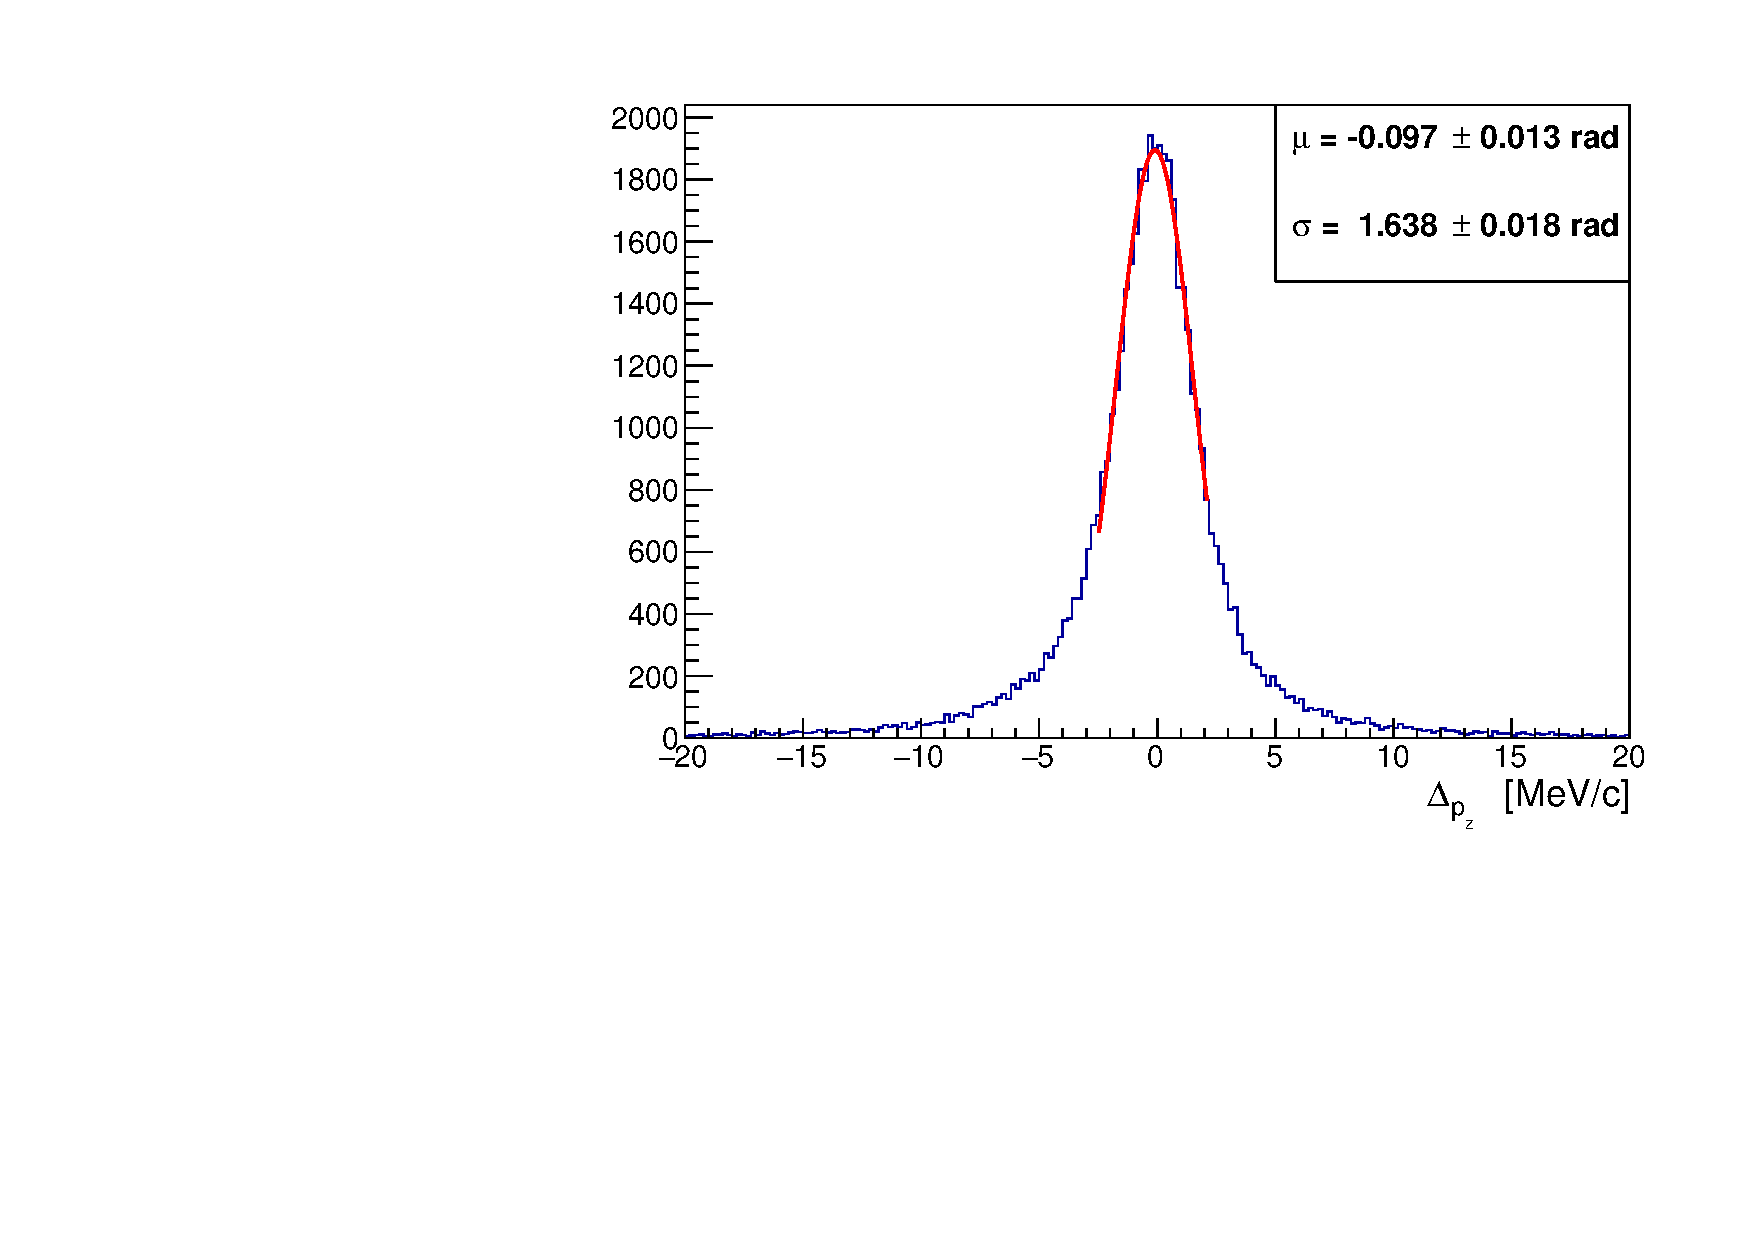
\includegraphics[width=0.49\textwidth, angle=0]{08-Performance/upstream_pz_residual.pdf}
      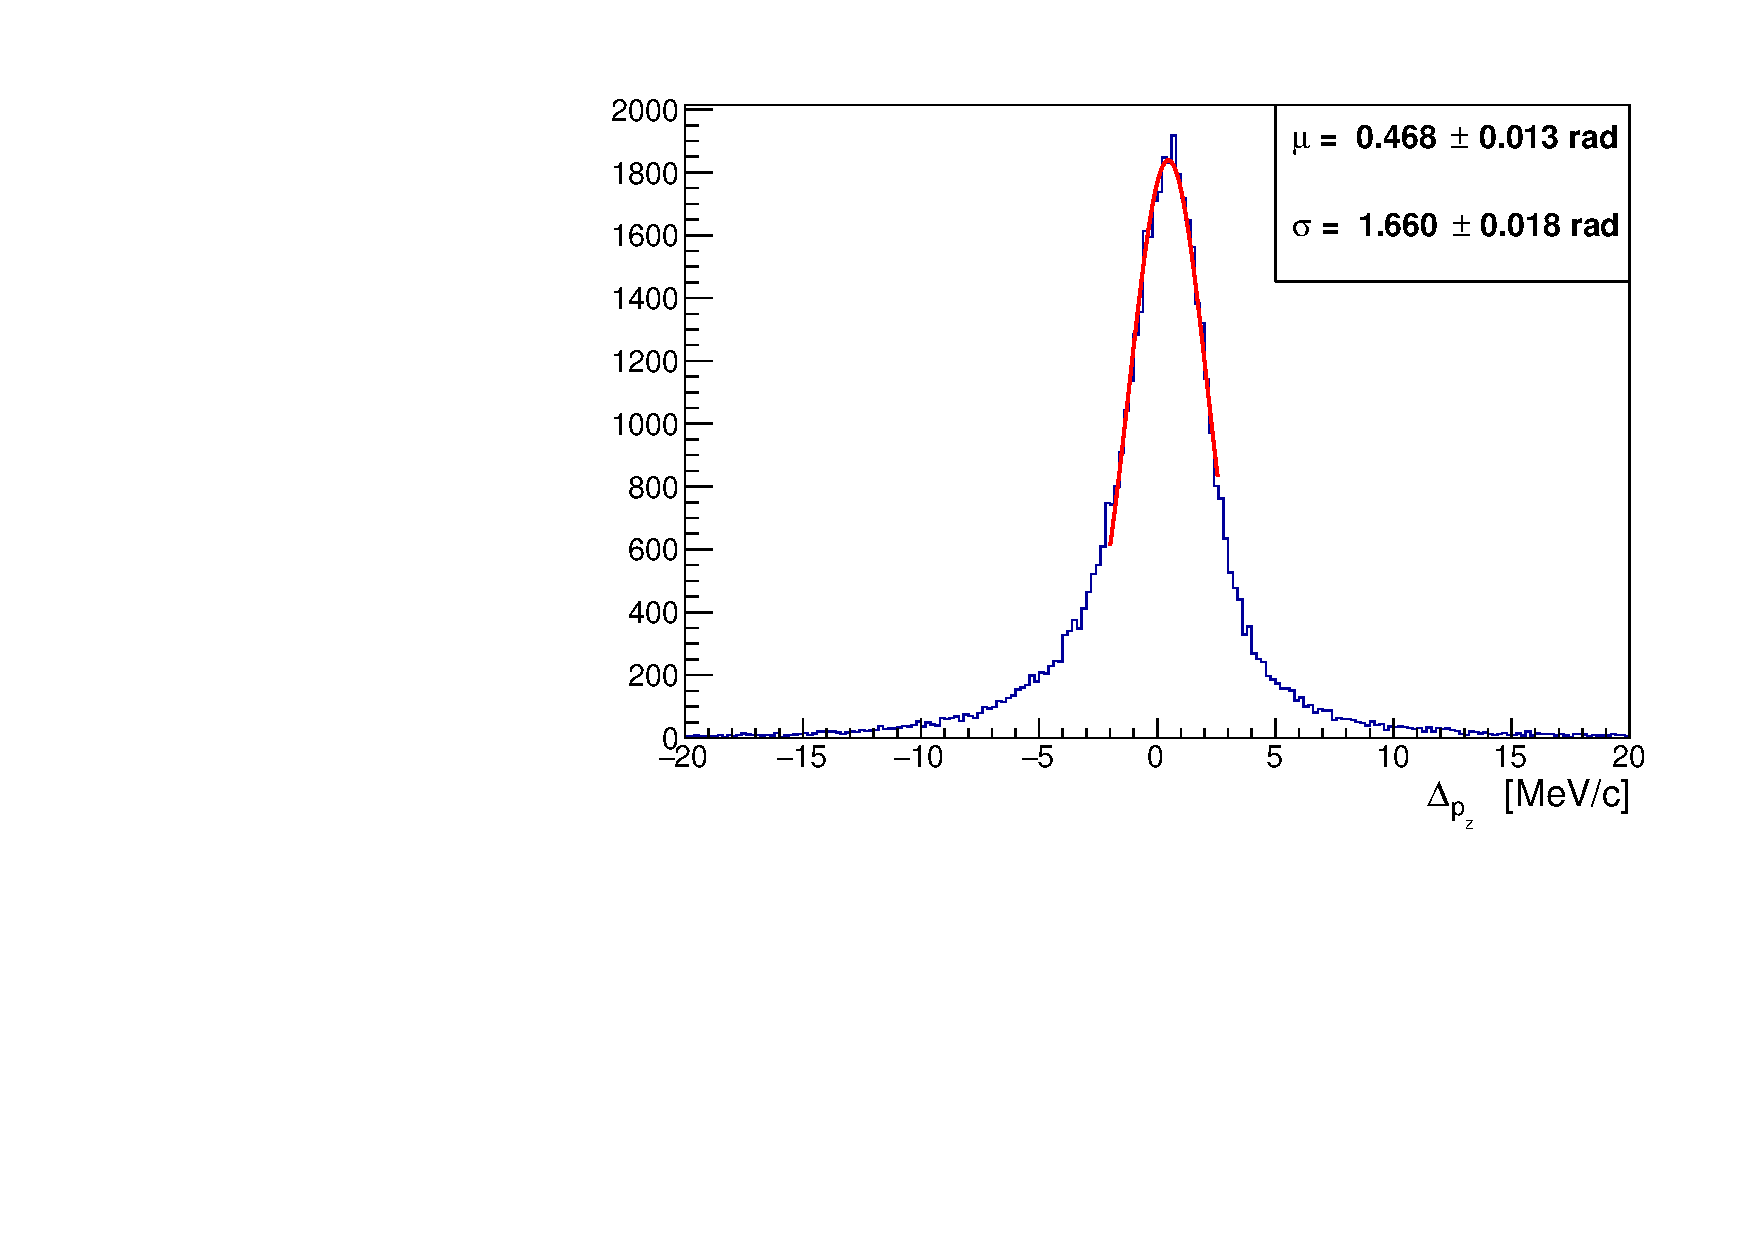
\includegraphics[width=0.49\textwidth, angle=0]{08-Performance/downstream_pz_residual.pdf}
      \caption{\label{fig:PzResidKalman} The $p_z$ residuals of the upstream (left) and downstream (right) trackers.}
    \end{center}
  \end{figure}
  
  \begin{figure}[p]
   \begin{center}
     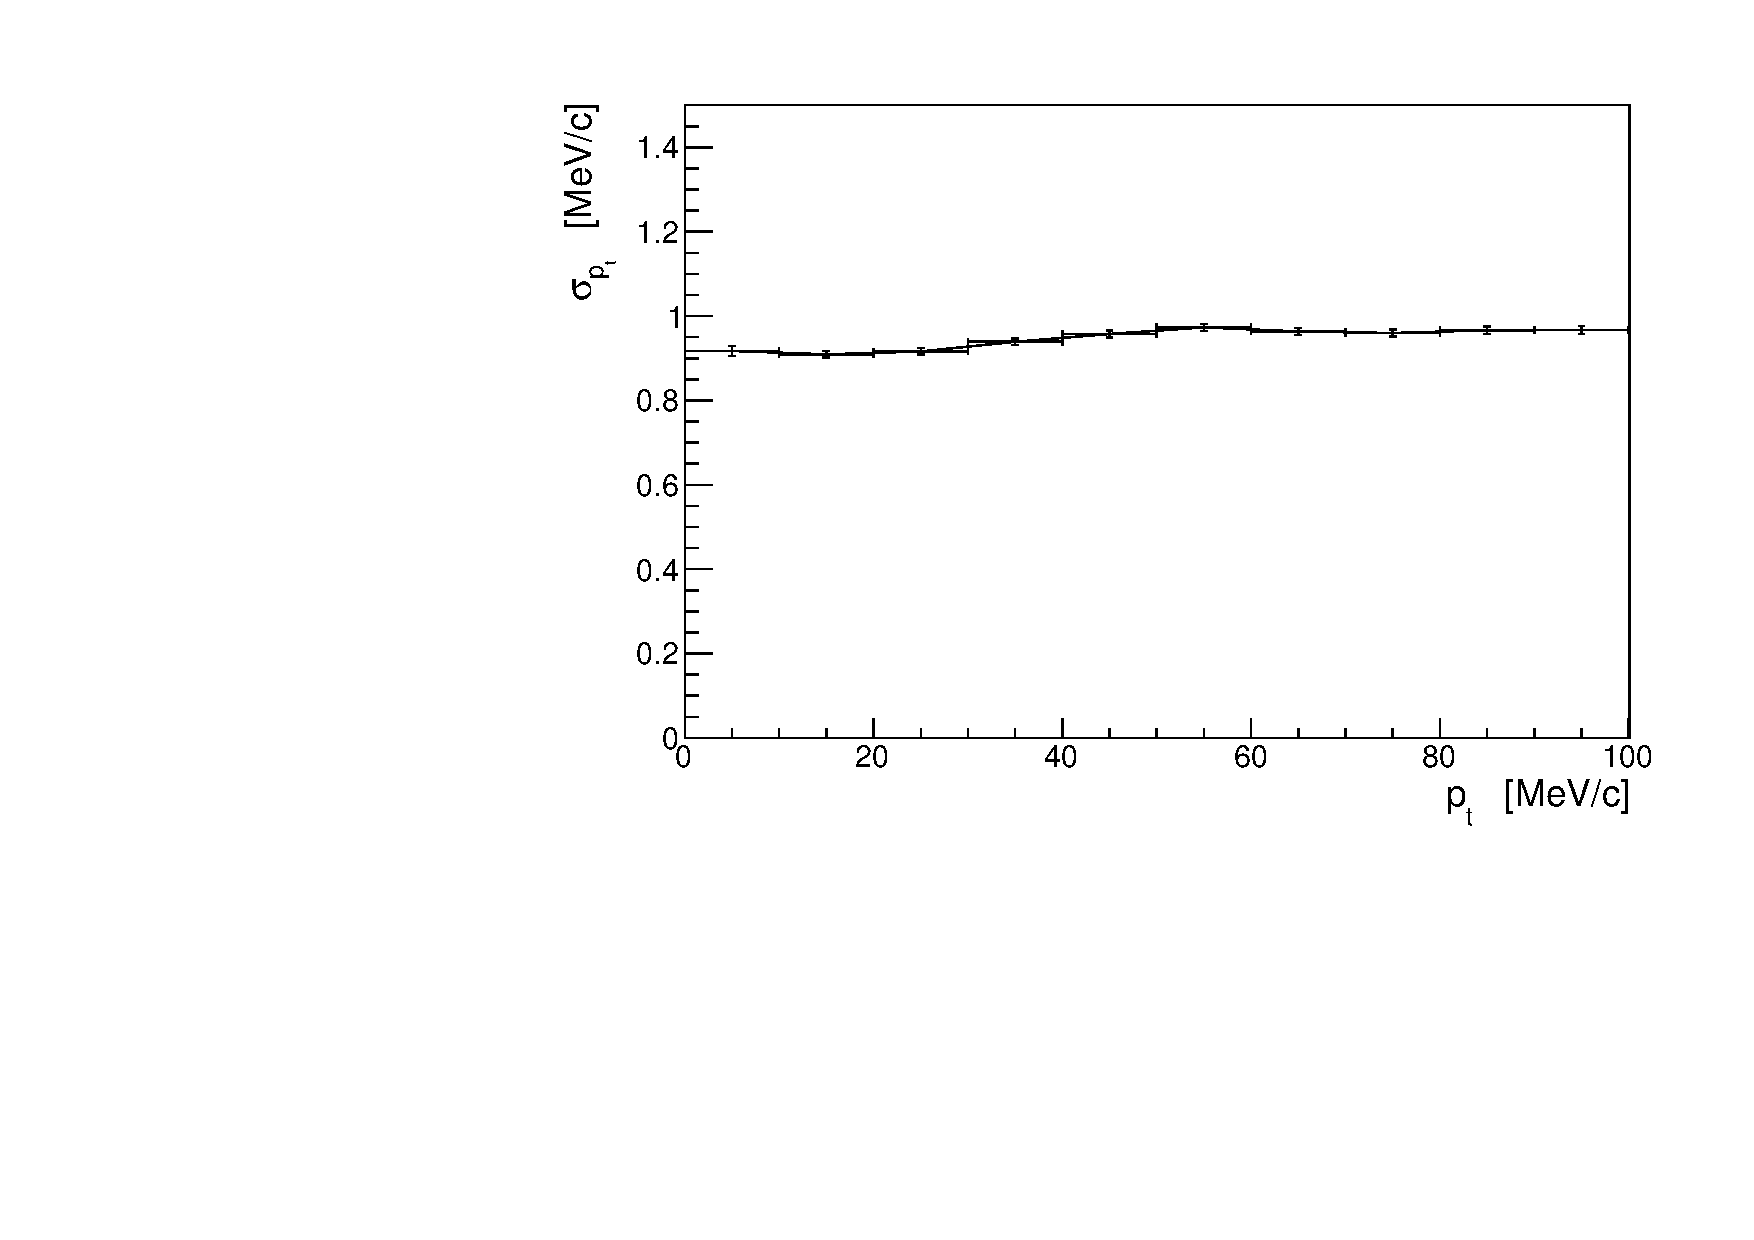
\includegraphics[width=0.49\textwidth, angle=0]{08-Performance/upstream_pt_resolution_pt.pdf}
     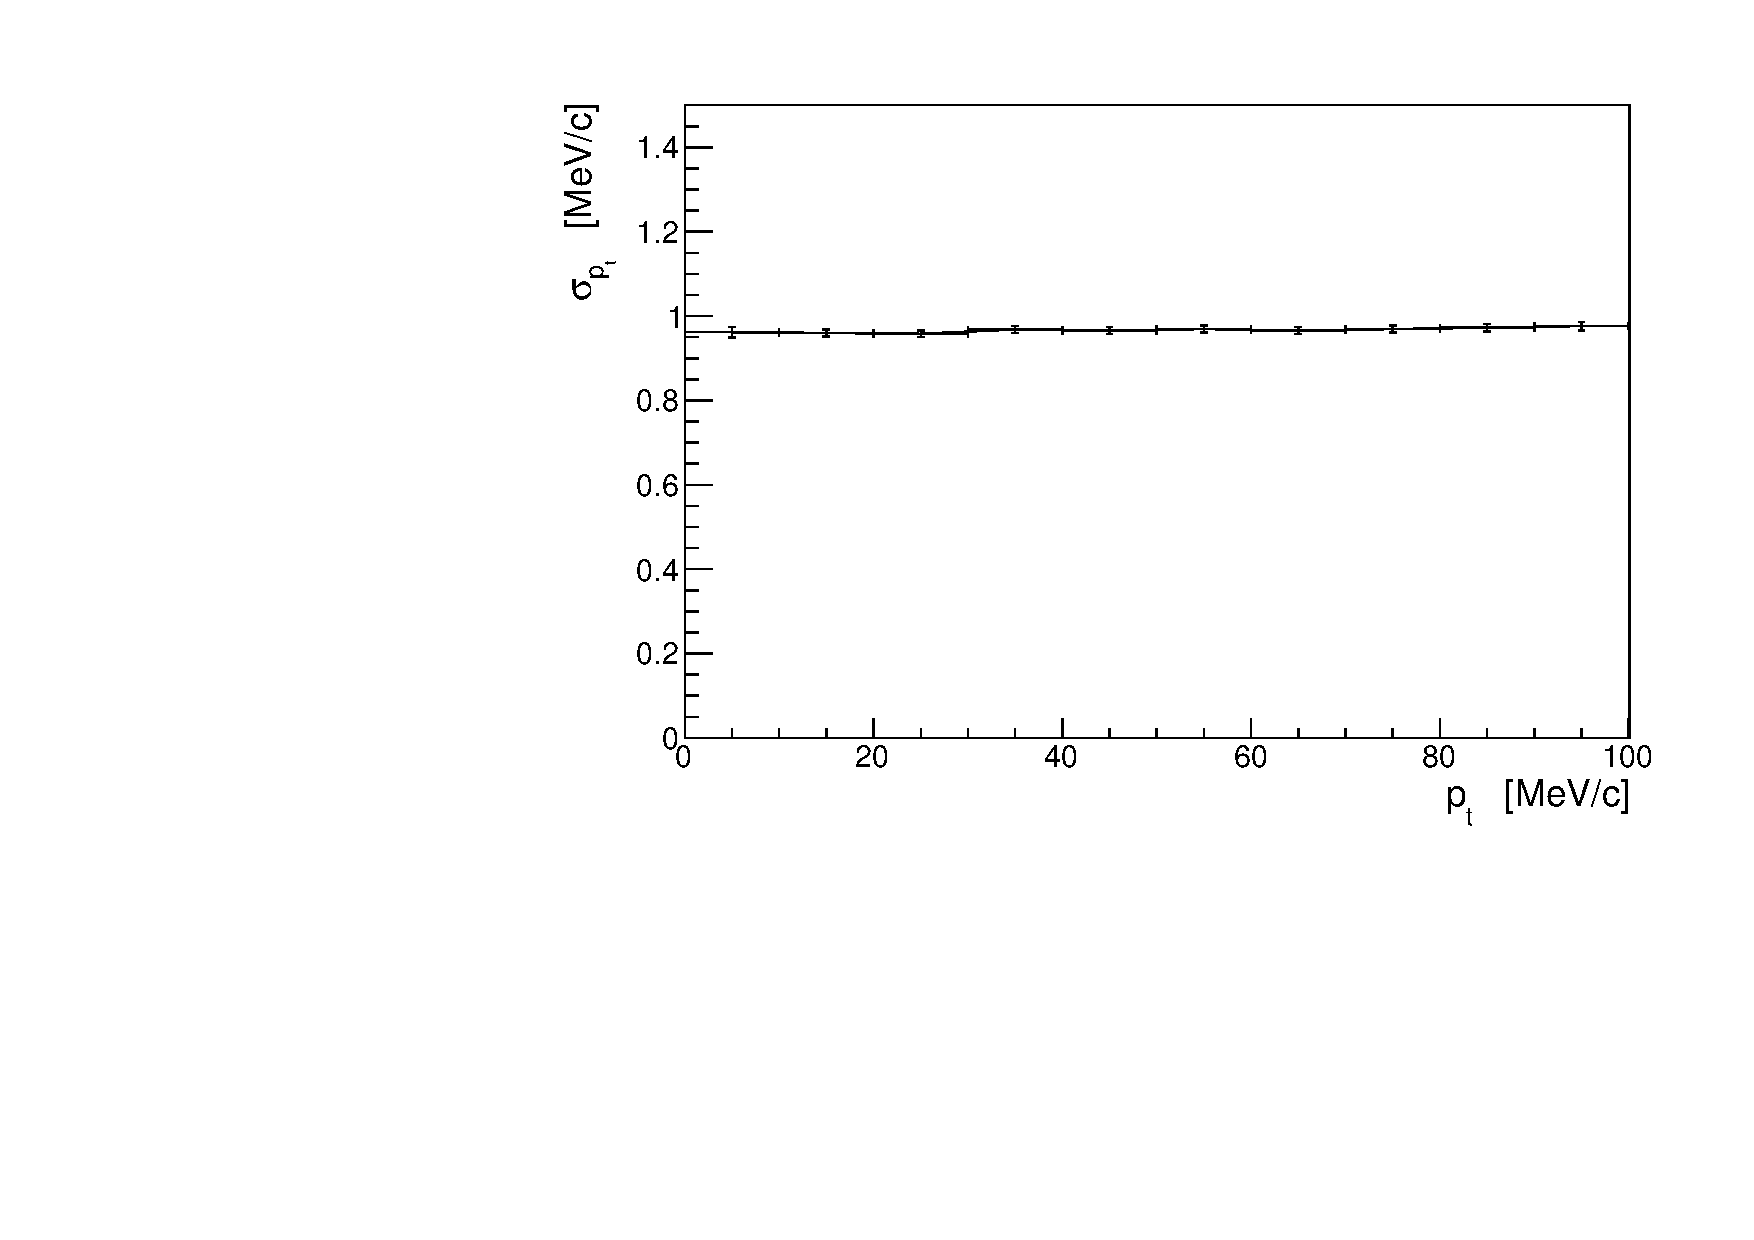
\includegraphics[width=0.49\textwidth, angle=0]{08-Performance/downstream_pt_resolution_pt.pdf}
     \caption{\label{fig:PtPtResolKalman} The $p_{t}$ resolution as a function of the $p_{t}$ of the upstream (left) and downstream (right) trackers.}
   \end{center}
  \end{figure}
  
  \begin{figure}[p]
   \begin{center}
     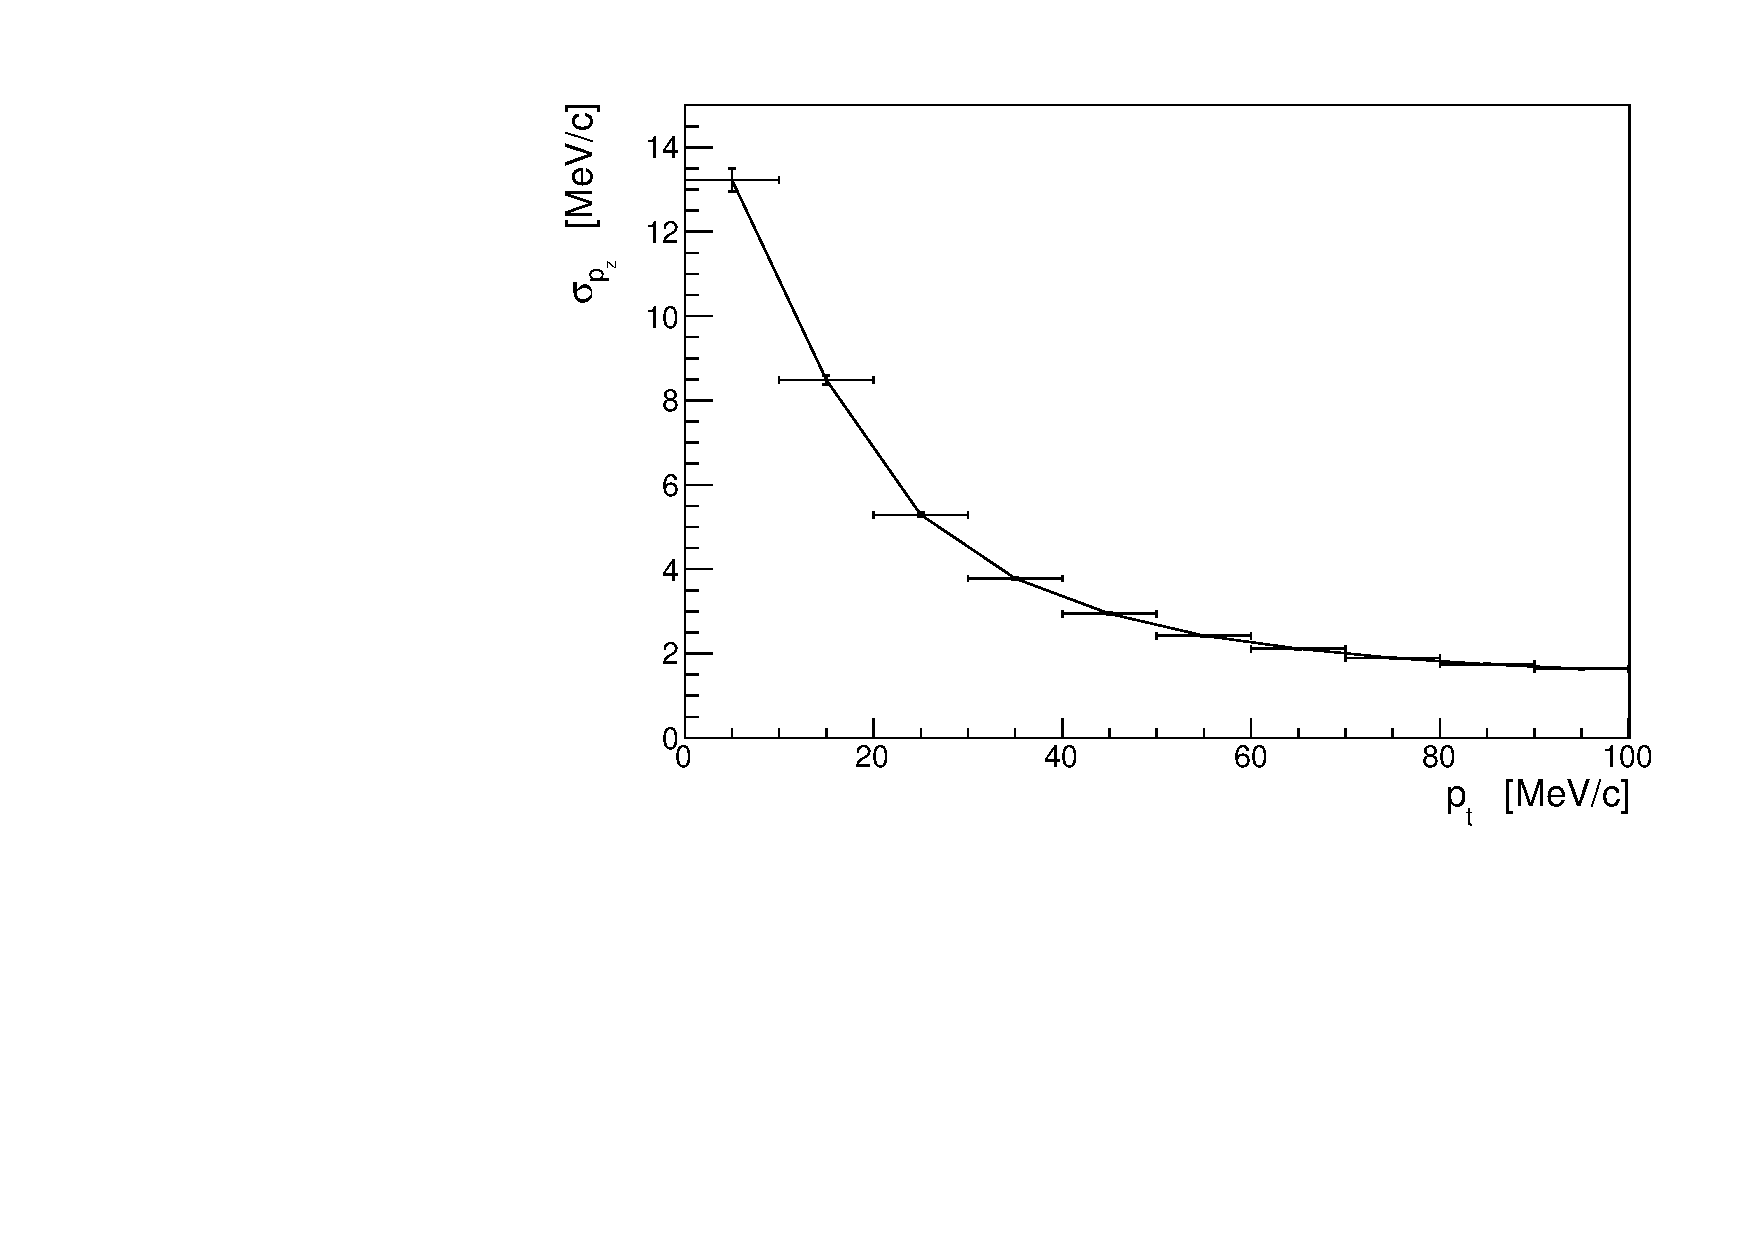
\includegraphics[width=0.49\textwidth, angle=0]{08-Performance/upstream_pz_resolution_pt.pdf}
     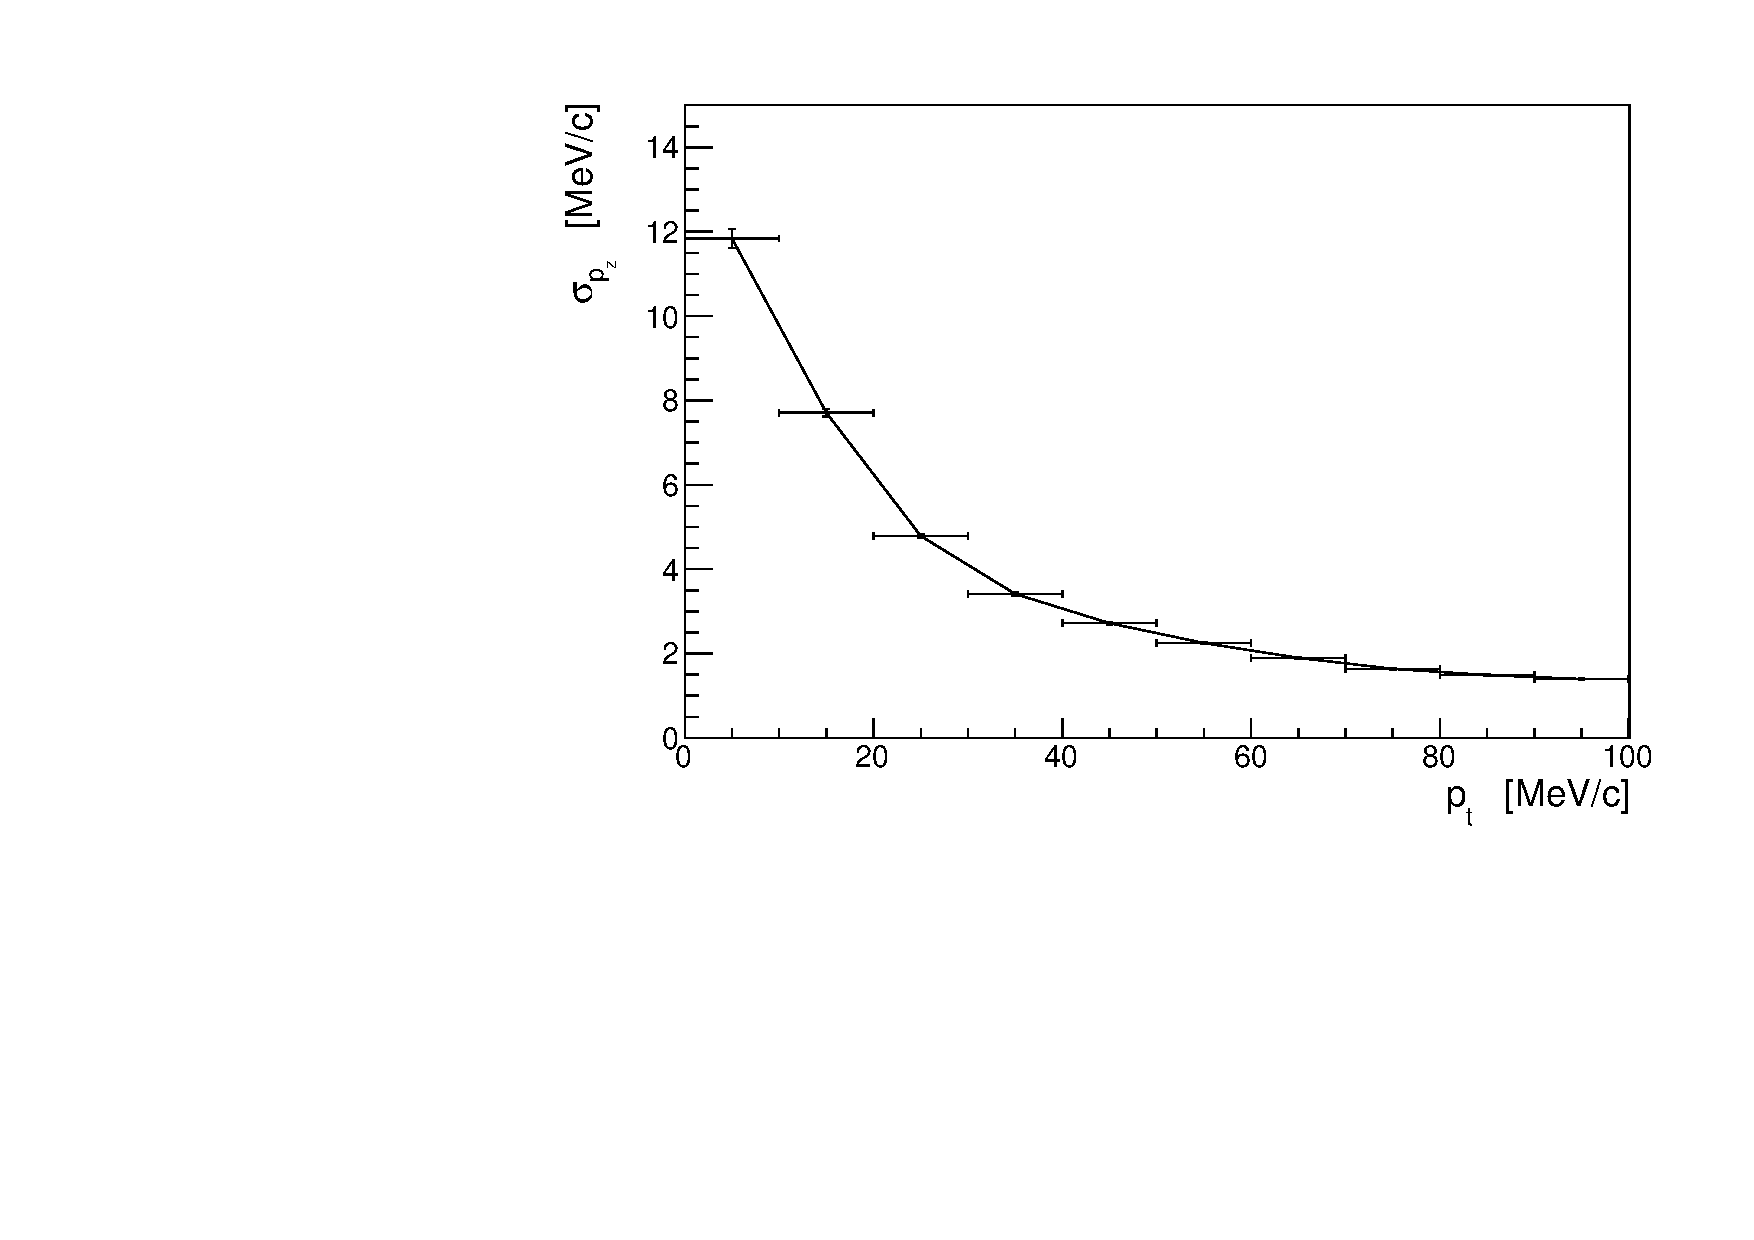
\includegraphics[width=0.49\textwidth, angle=0]{08-Performance/downstream_pz_resolution_pt.pdf}
     \caption{\label{fig:PtPzResolKalman} The $p_z$ resolution vs the $p_{t}$ of the upstream (left) and downstream (right) trackers.}
   \end{center}
  \end{figure}

